% Maga 4K mouse skull microCT -- pipeline migration validation.
% Build:
%   pdflatex manuscript
%   pdflatex manuscript

\documentclass{compactarticle}

\usepackage{amsmath,amssymb,amsfonts,bm}
\usepackage{graphicx}
\usepackage[utf8]{inputenc}
\usepackage[T1]{fontenc}
\usepackage{booktabs}
\usepackage{enumitem}
\usepackage{xcolor}
\usepackage{float}
\usepackage{ragged2e}
\usepackage{url}

\graphicspath{{figures/}}

\providecommand{\br}{\toprule}
\providecommand{\mr}{\midrule}

\begin{document}
\justifying
\fancyhead[R]{\small\itshape Maga 4K skull migration}

\articletype{Validation report}

\title{Migrating the 15\,MHz transcranial mouse pipeline from DigiMouse to
       the Maga (UW) 4K microCT: orientation, cavity extraction, and
       focal-prediction validation}

\author{Gianmarco F Pinton}

\affil{Joint Department of Biomedical Engineering, University of North
       Carolina at Chapel Hill and North Carolina State University}

\email{gia@email.unc.edu}

\keywords{transcranial focused ultrasound, mouse, microCT, skull,
          angular spectrum, Allen CCFv3}

\begin{abstract}
We document the migration of the 15\,MHz transcranial mouse corpus-callosum
therapy pipeline from the DigiMouse atlas (100\,$\mu$m isotropic, n=1
nude male) to the Maga laboratory (UW) 4K dry-skull microCT
(6.127\,$\mu$m isotropic, Skyscan 1272). At 15\,MHz the wavelength in
cortical bone is 176\,$\mu$m; DigiMouse provides $\sim$1.7\,voxels per
wavelength against $\sim$28 in the Maga 4K source data, and
$\sim$7\,voxels per wavelength at the 25\,$\mu$m working cache the
slab loader actually samples -- still a $\sim$4$\times$ improvement
over DigiMouse and the difference between a smoothed and a fully
resolved skull surface for angular-spectrum and FDTD propagation. This report
records the orientation determination from raw bone-mass profiles,
the streaming downsample to the 200\,$\mu$m ANTs cache, the simplified
endocranial-cavity extraction (dry skull, no jaw/spine sealing), the
ANTs-SyN registration of Allen CCFv3 to that cavity, the acoustic-property
mapping in the absence of a hydroxyapatite phantom, and a side-by-side
comparison of predicted focal pressure and aberration against the
DigiMouse baseline. Source data is reproducible: the Maga zip is
staged with \texttt{tuba.data.fetch\_mouse}; the Maga processing
pipeline (orientation, alignment, cavity extraction, SyN registration,
slab loading, bowl placement) lives at \texttt{src/tuba/species/mouse.py}
with intermediate caches in \texttt{\$TUBA\_MOUSE\_REG\_DIR}. The
DigiMouse baseline used for the comparison in \S\ref{sec:comparison} is
the legacy \texttt{mouse\_therapy/registration/} implementation (not
ported into TUBA).
\end{abstract}

% =============================================================================
\section{Source data}
\label{sec:source}

The Maga laboratory at the University of Washington has made
available a high-resolution microCT scan of an adult mouse dry skull
acquired on a Bruker Skyscan 1272 using a 4K detector~\cite{maga-uw}.
The reconstruction parameters embedded in the scan log are summarised
in Table~\ref{tab:scan-params}; the scan was acquired at 70\,kV /
142\,$\mu$A with an Al 0.5\,mm filter, oversampling in $0.1^\circ$
rotation steps over a 187.8$^\circ$ angular range, and reconstructed
with NRecon on GPU at 6.127\,$\mu$m isotropic voxel pitch. The volume
contains 3882 reconstructed axial TIFF slices of $2596 \times 1908$
pixels each, encoded uint16; the slice axis spans 23.8\,mm
(rostro-caudal extent of an adult mouse cranium), the row axis
$\sim$15.9\,mm (left-right width), and the column axis $\sim$11.7\,mm
(dorso-ventral height). The reconstructed volume is dry skull only --
no surrounding soft tissue and no in-situ brain. The unpacked TIFF
stack occupies $\sim$38\,GB; the compressed Box.com archive is
$\sim$5.7\,GB.

\begin{table}[H]
\centering
\caption{Maga 4K skull scan parameters (from embedded NRecon log).}
\label{tab:scan-params}
\small
\begin{tabular}{ll}
\toprule
Parameter & Value \\
\midrule
Source voltage (kV) & 70 \\
Source current ($\mu$A) & 142 \\
Filter & Al 0.5mm \\
Detector & PHOTONIC SCIENCE PS52 \\
Voxel pitch ($\mu$m) & 6.126685 \\
Angular range ($^\circ$) & 187.80 \\
Rotation step ($^\circ$) & 0.100 \\
Source--detector distance (mm) & 278.92879 \\
Source--specimen distance (mm) & 187.79218 \\
Reconstruction filter & Hamming (Alpha=0.54) \\
Recon time per slice (s) & 0.118496 \\
\bottomrule
\end{tabular}

\end{table}

\paragraph{Comparison with the DigiMouse baseline.} The DigiMouse
atlas~\cite{digimouse} provides a coregistered whole-body $380 \times 992
\times 208$ volume at 100\,$\mu$m isotropic from a single nude male
adult, including soft-tissue contrast (from cryosection-aligned CT)
and PET. The legacy DigiMouse pipeline in
\texttt{mouse\_therapy/\allowbreak registration/\allowbreak mouse\_ct\_constants.py}
(not ported into TUBA; retained as the comparison baseline)
resamples this to
200\,$\mu$m for ANTs ingest. The Maga 4K scan replaces the DigiMouse
CT specifically for skull modeling: it carries no soft tissue but
delivers a $\sim$16$\times$ refinement in linear voxel pitch.
Table~\ref{tab:source-compare} summarises the two sources side-by-side
under the 15\,MHz wavelength criterion.

\begin{table}[H]
\centering
\caption{DigiMouse vs Maga 4K microCT for 15\,MHz transcranial modeling.
Wavelength in cortical bone at 15\,MHz, assuming the conservative
mid-mineral cortical sound speed $c_{\mathrm{bone}}=2640$\,m/s, is
$\lambda_{\mathrm{bone}} \approx 176$\,$\mu$m. The acoustic-property
ramp of \S\ref{sec:acoustic-mapping} uses the higher-mineral
endpoint $c_{\mathrm{bone}}=2900$\,m/s for the cortical-bone anchor
(giving $\lambda_{\mathrm{bone}}\approx 193$\,$\mu$m there); the
sampling criterion in this table is anchored on the lower-velocity
end of the cortical range to keep the voxels-per-$\lambda$ count
conservative.}
\label{tab:source-compare}
\small
\begin{tabular}{lll}
\toprule
Property & DigiMouse & Maga 4K \\
\midrule
Voxel pitch ($\mu$m, isotropic) & 100 & 6.127 \\
Matrix size (i $\times$ j $\times$ k) & $380 \times 992 \times 208$ & $2596 \times 3882 \times 1908$ \\
Field of view (mm$^3$) & $38.0 \times 99.2 \times 20.8$ & $15.9 \times 23.8 \times 11.7$ \\
Coverage & whole body & head only (dry skull) \\
Soft tissue / in-situ brain & yes (cryosection-coreg) & no \\
HU / mineral-density calibration & yes & no (raw NRecon units) \\
Voxels per $\lambda_{\mathrm{bone}}$ at 15\,MHz & 1.76 & 28.7 \\
Specimens (n) & 1 (nude male, 28 g) & 1 \\
Native file size & 78\,MB & $\sim$38\,GB (uint16 stack) \\
\bottomrule
\end{tabular}

\end{table}

\paragraph{Native-resolution showcase.} Fig.~\ref{fig:native} shows
three orthogonal sections through the Maga 4K skull at the native
6.127\,$\mu$m voxel pitch, sampled from the aligned native volume of
\S\ref{sec:align} at the cavity centroid found in \S\ref{sec:cavity}.
After the pre-alignment the cavity centroid is essentially at the
midline ($x = +0.17$\,mm), so the sagittal section captures the dorsal
parietal vault as a thin ($\sim$200\,$\mu$m) trabecular shell, the
ventral palate and zygomatic process, and the densely septated nasal
turbinates at the rostral pole. The coronal section through the
cranium (at $y{=}{-}3.98$\,mm A-P) shows the inner table of the bone
shell with trabecular spaces visible across the entire wall thickness
and the complex basicranial processes (basisphenoid, vomer, palate
roots). The axial section just dorsal of the volume midplane
($z{=}{+}0.73$\,mm) captures the anterior nasal cavity with
individual turbinate plates and the posterior cranial cavity outline
in the same slice. Each PDF panel is rasterized at 1200\,dpi so the
full $\sim$3000$\,\times\,$2000 native pixel grid is preserved.

\begin{figure}[p]
\centering
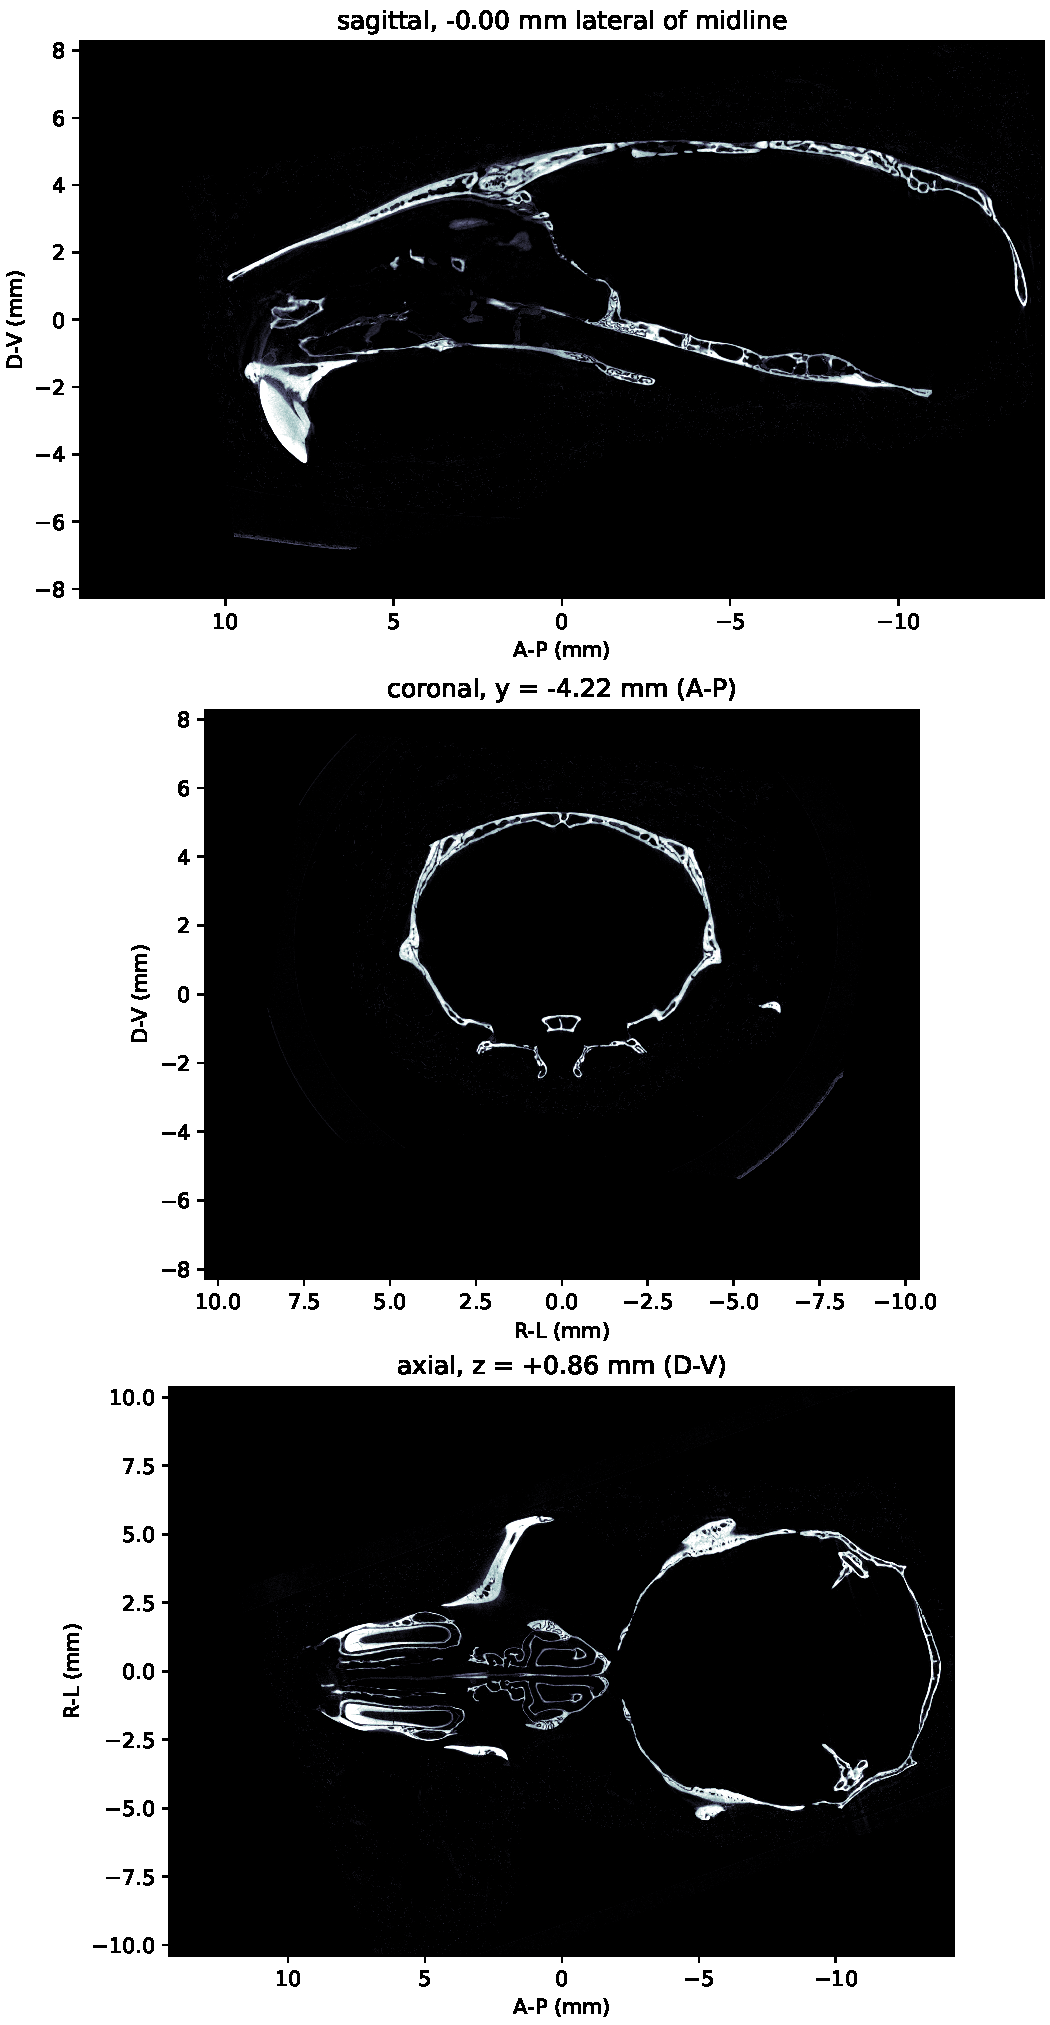
\includegraphics[width=0.85\textwidth,keepaspectratio]{native_orthoslices.pdf}
\caption{Native 6.127\,$\mu$m orthoslices through the aligned Maga 4K
         skull at the cavity centroid (top to bottom: sagittal at
         $+0.17$\,mm lateral of midline, coronal at $y{=}{-}3.98$\,mm
         A-P, axial at $z{=}{+}0.73$\,mm D-V). Intensities are
         percentile-clipped at [0.5\,\%, 99.5\,\%] for display. Each
         panel is rendered at 1200\,dpi to preserve the native pixel
         grid (underlying PNGs are $3882{\times}1908$ sagittal,
         $2596{\times}1908$ coronal, $2596{\times}3882$ axial).
         Anatomical features that DigiMouse cannot resolve at
         100\,$\mu$m -- ethmoid turbinates, the thin parietal vault
         cortex, sutures, and the internal trabecular spaces of the
         petrosal and basisphenoid -- are clearly visible.}
\label{fig:native}
\end{figure}

% =============================================================================
\section{Allen CCFv3 reference brain template}
\label{sec:allen}

The brain anatomy used throughout this pipeline is provided by the
Allen Common Coordinate Framework v3 (CCFv3), an averaged in-vivo
adult-mouse template derived from $\sim$1{,}675 specimens and
distributed by the Allen Institute alongside a hierarchical
parcellation of $\sim$670 anatomical structures~\cite{allen-ccfv3}.
The template ships at three isotropic resolutions (10, 25, and
50\,$\mu$m); we cache the 10\,$\mu$m template and annotation locally as
\texttt{allen\_template\_10um.nii.gz} and
\texttt{allen\_annotation\_10um.nii.gz} (1140${\times}$1320${\times}$800
voxels, $\sim$11.4${\times}$13.2${\times}$8.0\,mm$^3$, RAS-affined) under
\texttt{\$TUBA\_MOUSE\_REG\_DIR} via
\texttt{tuba.data.fetch\_allen}, and use the 25\,$\mu$m
companion volumes as the moving/fixed images for the SyN registration
in \S\ref{sec:registration}.

Fig.~\ref{fig:allen} shows the Allen reference at its native
10\,$\mu$m resolution \emph{prior to any transformation} into Maga
skull space, in the same 3${\times}$2 (sag, cor, axi) ${\times}$ (template,
annotation) layout that the post-warp registration QC of
\S\ref{sec:registration} will reuse. The left column is the averaged
template intensity (greyscale) and the right column overlays the
anatomical annotation as one saturated colour per structure ID (the
three orthoslices intersect 374 distinct regions). Holding the
unwarped reference next to the warped result in
Fig.~\ref{fig:registration} lets the reader see by inspection that
the SyN deformation preserves the gross internal partitioning of the
atlas -- cortical mantle, hippocampus, thalamus and hypothalamus,
midbrain colliculi, cerebellum, and brainstem all retain their
relative positions and the gross shape of their boundaries -- while
the outer contour conforms to the actual endocranial cavity of the
Maga 4K skull.

\begin{figure}[p]
\centering
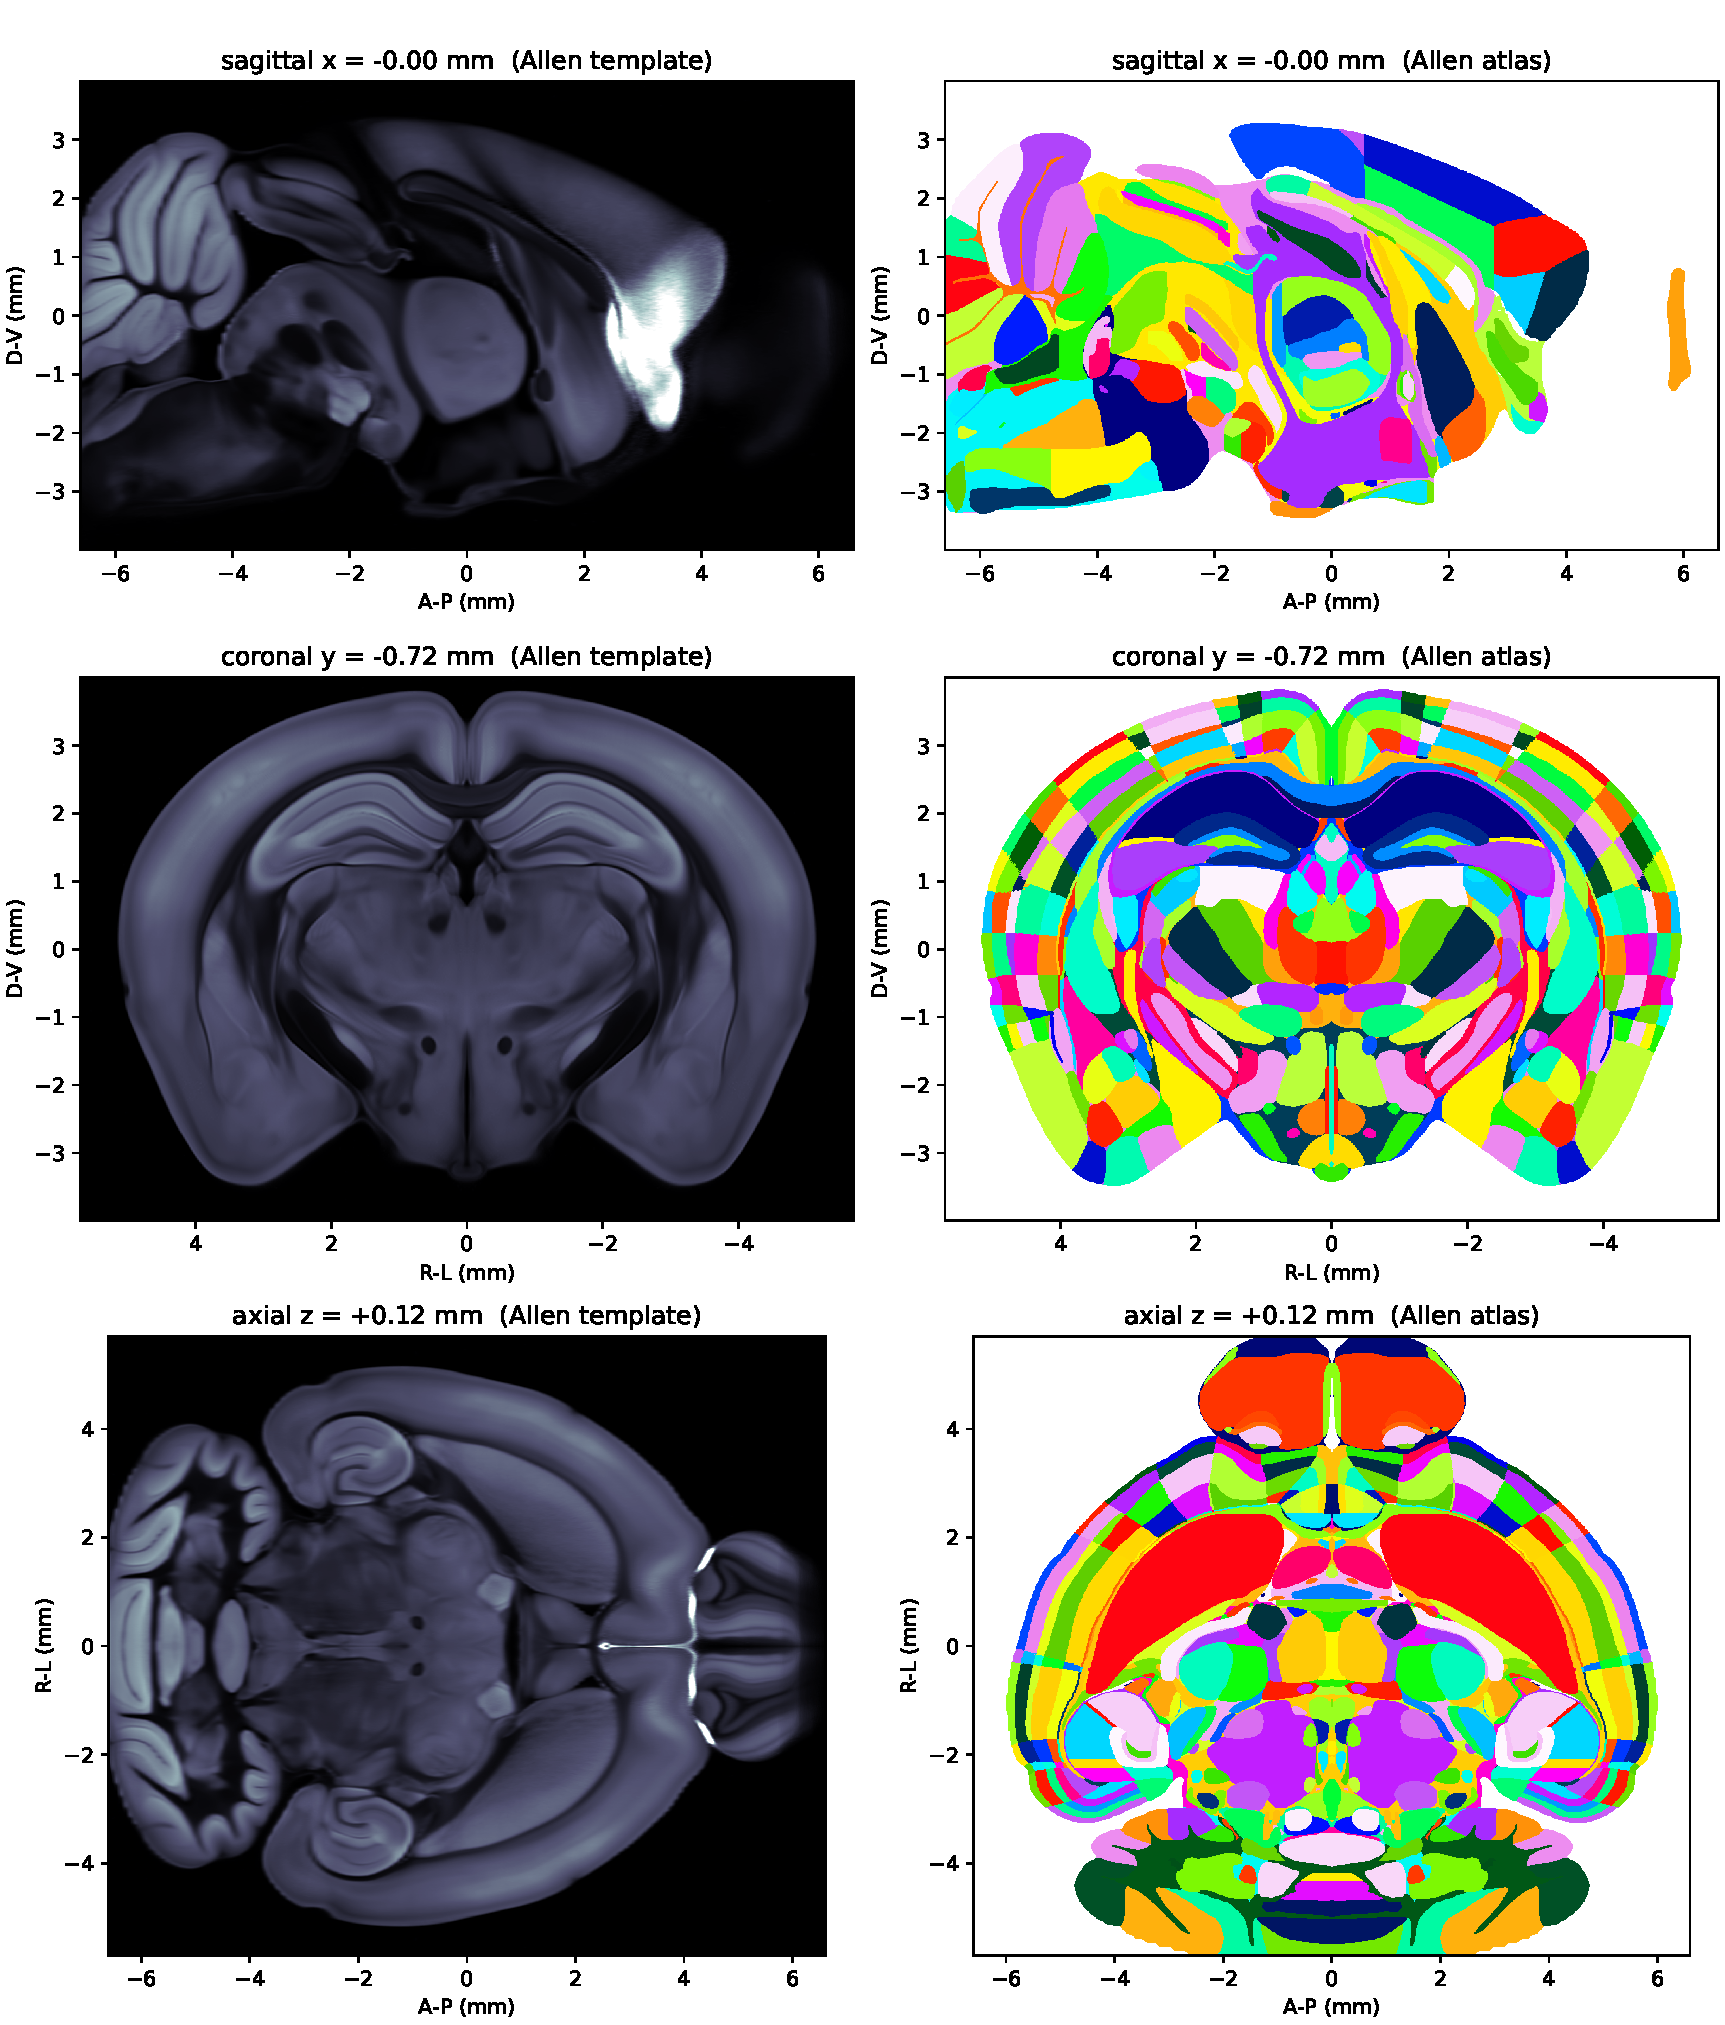
\includegraphics[width=\textwidth,keepaspectratio]{allen_reference.pdf}
\caption{Allen CCFv3 reference at native 10\,$\mu$m resolution,
         pre-warp. Three orthoslices (sagittal, coronal, axial, top
         to bottom) through the brain mass centroid
         ($x{=}-0.005$\,mm, $y{=}-0.73$\,mm, $z{=}+0.11$\,mm in the
         Allen world frame). \textbf{Left column}: averaged template
         intensity at percentile-clipped greyscale, showing the
         smooth ex-vivo MR-style contrast that the SyN registration
         matches against the binarised endocranial cavity. \textbf{Right
         column}: anatomical annotation atlas, each Allen structure
         ID rendered in a distinct saturated colour from the
         \texttt{gist\_ncar} palette (deterministic ID${\to}$hue
         shuffle so neighbouring IDs are well-separated). The same
         orthoslice layout reappears at the same world coordinates
         (relative to the cavity centroid) after the SyN warp in
         Fig.~\ref{fig:registration}.}
\label{fig:allen}
\end{figure}

% =============================================================================
\section{Orientation determination}
\label{sec:orientation}

The Maga TIFF stack carries no DICOM or NIfTI affine; the only
reconstruction metadata is the per-slice in-plane pixel pitch. To
determine the mapping from storage axes $(s, r, c)$ to anatomical
$(R\text{-}L, A\text{-}P, D\text{-}V)$ we sampled 21 evenly spaced
slices through the stack and computed (i) total bone-voxel count
per slice using a uint16 threshold of 8000, (ii) the row and column
centroid of bone within each slice, and (iii) the bone bounding box
within each slice.

The per-slice bone-mass profile (Fig.~\ref{fig:orientation-profile})
is bell-shaped with two narrow tails: bone first appears near storage
slice 100, the cross-section grows monotonically, peaks at storage
slice $\sim$2383 ($\sim$295k bone voxels), and after a moderate decline
shows a secondary peak near storage slice $\sim$3570 ($\sim$245k
bone voxels) just before collapsing to zero. The total slice-axis
extent ($3882 \times 6.127\,\mu$m $= 23.8$\,mm) matches the canonical
adult mouse skull length, confirming that the slice axis is
rostro-caudal.

Bone-mass alone is ambiguous as to which end of the slice axis is
rostral: both interpretations (slice 0 = rostral or slice 0 = caudal)
predict a narrow tail, a gradual rise, a broad peak, and a sharp
secondary peak near the other end. This is disambiguated by direct
inspection of the native-resolution orthoslices in
Fig.~\ref{fig:native}: the sagittal section shows the nasal turbinates
at positive $y$ and the brain compartment as a smooth oval cavity at
negative $y$, and the axial section shows the same arrangement (intricate
turbinate bone at $+y$, smooth cranial outline at $-y$). The slice
axis is therefore flipped in
\texttt{tuba.species.mouse} (\texttt{SLICE\_FLIP = True}) so that the
RAS-aligned NIfTI satisfies the convention
$+y = \mathrm{anterior}$. The secondary bone-mass peak at storage
slice $\sim$3570 corresponds anatomically to the dense incisor /
ethmoid-turbinate region just caudal of the rostral tip.

The in-plane axes have lengths $2596 \times 6.127\,\mu$m $= 15.9$\,mm
and $1908 \times 6.127\,\mu$m $= 11.7$\,mm; these match the expected
left-right width and dorso-ventral height of a mouse skull. The D-V
sign was disambiguated by the bone-mass-per-slice distribution along
the column (D-V) axis of the 200\,$\mu$m cache: the lowest-$k$ slices
($k=0\dots4$) contain zero cortical-bone voxels, while the highest-$k$
slices ($k=52\dots56$) contain 272, 164, 61, 39, 41 cortical-bone
voxels respectively. The only structure with this density profile is
the basicranium (palate, basisphenoid, petrosal), which is
anatomically ventral. Storage high-$k$ therefore corresponds to
ventral, and \texttt{COL\_FLIP = True} is set in
\texttt{tuba.species.mouse} so that the output volume satisfies
$+z = \mathrm{dorsal}$ in RAS. A naive bone-vs-cavity centroid test
gives a misleading positive ($z_{\mathrm{cavity}} - z_{\mathrm{bone}} =
+0.5$\,mm) because the brain cavity occupies the upper-middle of the
skull while the bone-centre falls just below it, almost regardless of
flip sign; only the per-$k$ bone-mass tail behaviour is decisive.

The L-R sign is left at its default (storage row 0 $\to$ right-most)
since the skull is approximately L-R symmetric and direct visual
verification is not possible from the unregistered volume alone; any
residual L-R mirror will be caught by the Allen CCFv3 registration
(\S\ref{sec:registration}).

\begin{figure}[H]
\centering
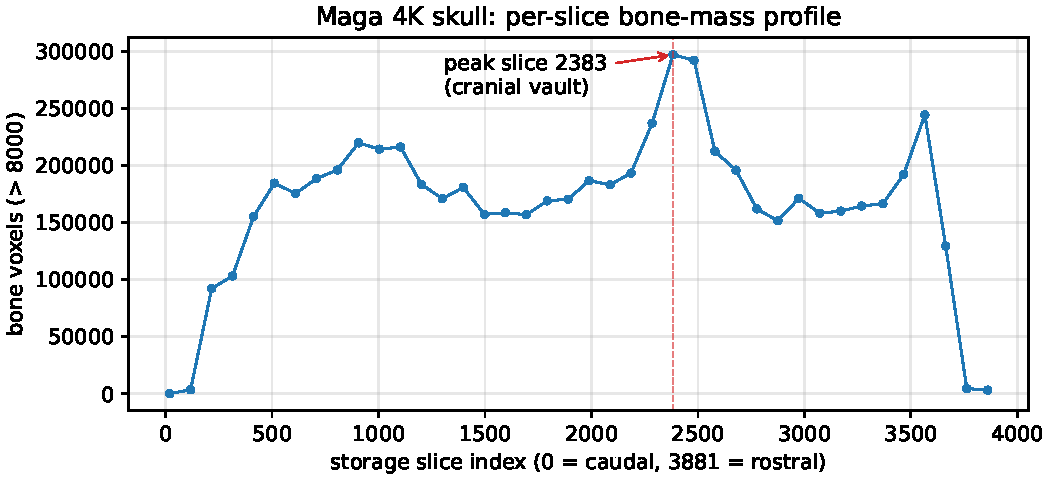
\includegraphics[width=0.85\linewidth]{orientation_profile.pdf}
\caption{Per-slice bone-mass profile across the 3882-slice Maga 4K stack
         (uint16 threshold 8000). The bell-shaped profile peaks at
         storage slice $\sim$2383 (cranial vault) and shows a secondary
         peak at storage slice $\sim$3570 corresponding to the dense
         incisor / ethmoid region near the rostral tip. The total
         slice-axis extent (23.8\,mm) matches an adult mouse skull
         length and confirms the slice axis is rostro-caudal. The
         direction (storage 0 = caudal, storage 3881 = rostral) is
         determined by the native orthoslice QC in
         Fig.~\ref{fig:native}, not by this profile.}
\label{fig:orientation-profile}
\end{figure}

% =============================================================================
\section{Downsampling to the 200\,$\mu$m ANTs cache}
\label{sec:downsample}

The native 6.127\,$\mu$m volume is too large for direct ANTs SyN
registration ($\sim$38\,GB float32). We provide a streaming
block-max downsampler that produces a clean RAS-affined NIfTI at any
target voxel pitch that is an integer multiple of the native pitch
(see \texttt{tuba.species.mouse.\allowbreak downsample\_to\_200um} /
\texttt{downsample\_to\_50um}). The default 200\,$\mu$m
cache uses a factor-of-33 reduction (200\,$\mu$m / 6.127\,$\mu$m $=
32.65$, rounded to 33, giving an actual pitch of 202.2\,$\mu$m); a
50\,$\mu$m cache (factor 8, $\sim$6\,GB float32) is also provided for
work that needs more detail than ANTs but less than native.

All downstream visualisations (cavity extraction, registration QC) are
rendered at the native 6.127\,$\mu$m pixel grid; the 200\,$\mu$m cache
is the moving image for ANTs SyN, and the 25\,$\mu$m cache is the
target grid for the inverse-warped Allen template and annotation. In
the QC figures, each volume is plotted at its own world-coordinate
extent (via the NIfTI affine), so the three pixel grids (native skull,
200\,$\mu$m cavity contour, 25\,$\mu$m warped Allen) overlay without
explicit resampling.

% =============================================================================
\section{Rigid pre-alignment to the storage axes}
\label{sec:align}

After the storage$\to$RAS axis flips of \S\ref{sec:orientation} the skull's
anatomical axes are still tilted with respect to the index axes: the
dorsal vault is not horizontal, the midsagittal plane is not exactly
perpendicular to the R-L index axis, and the rostro-caudal long axis is
rotated in the A-P/R-L plane. Working in tilted index space complicates
both the cavity extractor (which uses an axis-aligned bounding box for
the caudal foramen-magnum seal) and downstream acoustic simulations
(which assume that anatomical axes align with the FDTD grid). We
therefore apply a single rigid 3-D rotation to the 200\,$\mu$m cache
(and to the native volume; see \S\ref{sec:cavity}) before any further
processing.

The rotation is parameterised by three Euler angles in the intrinsic
ZYX convention,
\begin{equation}
R = R_z(\alpha_z)\,R_y(\alpha_y)\,R_x(\alpha_x),
\end{equation}
applied to column vectors in voxel-index space. Sign convention follows
the right-hand rule about each anatomical axis. The angles are derived
automatically from principal-component analysis (PCA) of the densest
cortical bone (intensity threshold $30{,}000$ on the uint16 NRecon
scale; selecting threshold high enough to exclude both the specimen
mount and the diffuse vault, so that PCA's covariance is dominated by
the well-defined bilateral dental arches and basicranial plates).
Eigenvectors of the centroid-centred bone cloud are assigned to the
target storage axes by descending variance:
\begin{itemize}
\setlength\itemsep{0pt}
  \item largest eigenvalue $\to$ A-P (the skull's $\sim$23.8\,mm long axis)
  \item middle eigenvalue $\to$ R-L (15.9\,mm width)
  \item smallest eigenvalue $\to$ D-V (11.7\,mm height)
\end{itemize}
A right-handed orthonormal frame $V = [\mathbf v_{RL}\,\mathbf v_{AP}\,
\mathbf v_{DV}]$ is constructed and the rotation $R = V^{\!\top}$ sends
$V$'s columns onto the storage basis. Closed-form ZYX decomposition of
$R$ yields the angles to apply via
\texttt{scipy.ndimage.affine\_transform}, and the same affine is
applied to the native TIFF stack to produce
\texttt{maga\_skull\_aligned\_native.\allowbreak nii.gz} (uint16,
streamed in memory; see
\texttt{align\_skull\_to\_axes} and \texttt{align\_native\_to\_axes} in
\texttt{tuba.species.mouse}). In the same step the cortical-bone
centroid is translated to the volume centre so the brain cavity sits at
the world origin. The output volume is padded by 12 voxels on each
side (200\,$\mu$m cache) or 396 voxels (native), so that
rotation+centring does not push the caudal extreme of the skull past
the output bounding box; without this pad, the foramen-magnum end of
the cavity gets clipped and the downstream caudal seal (\S\ref{sec:cavity})
becomes unreliable.

For the Maga scan the PCA-derived angles are
$(\alpha_x,\alpha_y,\alpha_z) = ({+}8.07^\circ,\,{+}8.40^\circ,\,
{-}19.51^\circ)$. The dorsal vault apex lands within
$\pm 0.5$\,voxel of the midsagittal plane after the rotation, the
basicranial plates are bilaterally symmetric about R-L${=}0$, and the
brain cavity centroid is centred at the world origin (sub-voxel
residual). Crucially, this anatomical pre-alignment is a one-shot
choice of coordinates -- it does not affect the SyN registration to the
Allen template, which finds its own optimum independently, but it makes
all downstream slice plots cleanly axis-aligned.

% =============================================================================
\section{Endocranial-cavity extraction (dry skull)}
\label{sec:cavity}

The DigiMouse cavity extractor
(legacy \texttt{mouse\_therapy/registration/\allowbreak extract\_mouse\_cavity.py};
not in TUBA) contains $\sim$300 lines and must solve several problems specific to
the whole-body scan: detecting the skull-base $k$ slice from the
contrast between vault and basal-skull bone fractions, plugging the
foramen magnum to seal the spinal column, and per-slice connected-component
filtering around an a~priori brain centre to suppress 2-D leakage into
the nasal sinuses, orbits, and oral cavity. None of these are needed
for the Maga dry skull -- the scan contains no spine, no mandible, no
soft tissue, and no body posterior to the occiput. We therefore
re-implement the extractor as
\texttt{tuba.species.mouse.\allowbreak extract\_cavity}.

The principal residual challenge is intensity-distribution shape. The
log-binned histogram of the native volume (Fig.~\ref{fig:histogram})
reveals three populations on the raw NRecon uint16 scale (\textbf{k\,cts}
$=10^3$ counts; no hydroxyapatite phantom calibration was applied, so
these are not Hounsfield units): air ($<100$, 19\,\% of voxels), a
broad plateau at 4--8\,k\,cts corresponding to the specimen-mounting
material that holds the dry skull in the scanner (50\,\% of voxels), and
true cortical bone at 20--40\,k\,cts (9\,\% of voxels). A single intensity
threshold cannot simultaneously yield a complete bone shell (which
requires including some of the 4--8\,k\,cts material to bridge thin
cortex and small foramina) and a faithful bone exclusion mask (which
must be restricted to the cortical-bone peak only). We therefore use
the hysteresis-threshold strategy of the DigiMouse extractor:

\begin{itemize}[leftmargin=*]
\item \texttt{BONE\_HIGH} $= 15000$: voxels above this are classified as
      cortical bone and excluded from the cavity mask.
\item \texttt{BONE\_LOW}  $= 5000$: voxels above this seed the shell
      that is dilated, then unioned with the caudal seal. The threshold
      is lowered from the legacy 6000 because the cache used here is
      block-max'd from the rotation-interpolated aligned native, whose
      order-1 interpolation softens cortical-bone intensities by
      $\sim$25\,\% relative to a raw-TIFF block-max; the histogram
      fraction above 5000 in the new (rotation-interpolated 25\,$\mu$m)
      cache (14.3\,\%) approximately matches the legacy fraction
      above 6000 in the raw-TIFF block-max 200\,$\mu$m cache
      (10.4\,\%).
\end{itemize}

\begin{figure}[H]
\centering
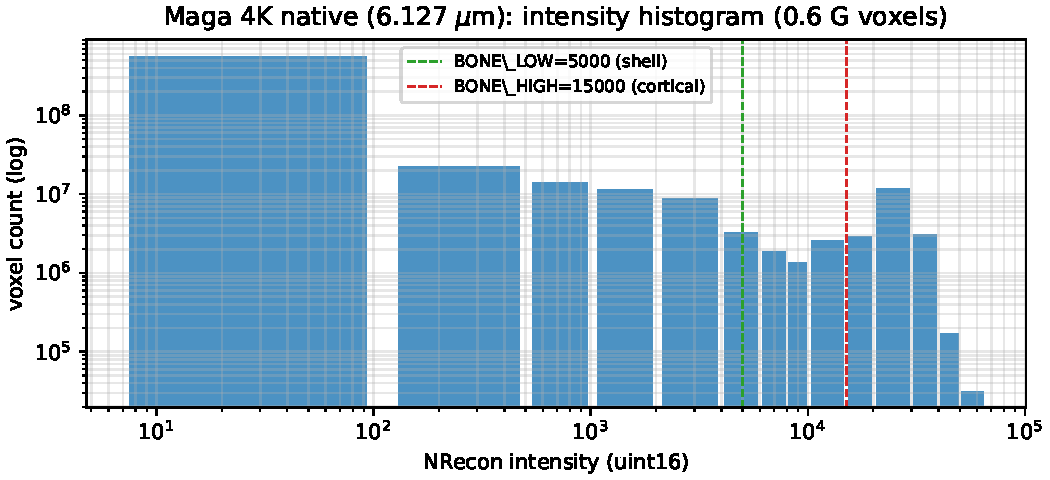
\includegraphics[width=0.85\linewidth]{intensity_histogram.pdf}
\caption{Log-binned intensity histogram of the Maga 4K volume,
         accumulated from a sample of every 33rd native 6.127\,$\mu$m
         TIFF slice ($\sim$0.6 G voxels total). Air, mounting material,
         and cortical bone form three distinct populations. The
         hysteresis thresholds \texttt{BONE\_HIGH=15000} and
         \texttt{BONE\_LOW=5000} fall within the gaps between
         populations.}
\label{fig:histogram}
\end{figure}

The pipeline:
\begin{enumerate}[leftmargin=*]
\item Build a caudal seal: at the most-caudal cortical-bone slice
      fill the $(i, k)$ bone bounding box with \texttt{True} over the
      most-caudal 0.6\,mm to plug the foramen magnum.
\item Build the shell: \texttt{binary\_closing} of the
      \texttt{BONE\_LOW} mask by 1.0\,mm (seals foramina up to $\sim$2\,mm
      diameter, covering the cribriform plate, optic canals, ear-bullae
      openings, and any sutural gaps), unioned with the caudal seal.
      Closing -- dilation followed by erosion at the same radius -- seals
      holes without the net inward boundary shift that a pure dilation
      would impose at this working resolution.
\item Identify outside-of-skull voxels by region-growing
      \texttt{$\sim$shell} from the volume border
      (\texttt{scipy.ndimage.label}, then keep every component touching
      the bounding box).
\item \texttt{cavity\_raw = \textasciitilde shell \& \textasciitilde outside} --
      every voxel inside the bone+mounting envelope that is not classified as
      shell.
\item Keep the largest connected component. This is the cerebrum +
      cerebellum + brainstem compartment ($\sim$450\,mm$^3$). The
      olfactory-bulb cavity ($\sim$50\,mm$^3$) appears as a separate CC
      because the closed cribriform plate now seals it from the main
      compartment; it is not retained as the moving image (preserving
      topological correspondence with the connected Allen brain mask),
      and the warped Allen template recovers the OB region via the
      SyN deformation field.
\end{enumerate}

The extractor is run on a 24.5\,$\mu$m cache built by factor-4 block-max
decimation of the \emph{aligned} native (6.127\,$\mu$m) volume rather
than from raw TIFFs followed by independent PCA alignment. Both
approaches put the volume centre at the world origin, but they centre
on different physical points: a 200\,$\mu$m cache built from raw TIFFs
and then PCA-rotated chooses its bone centroid after block-max has
smeared the 4--8\,k\,cts mounting-material plateau into apparent bone,
biasing the centroid ventrally by $\sim$1\,mm. Deriving the working
cache from the already-aligned native sidesteps this bias and ensures
that cavity, native skull, and downstream Allen overlays share an
identical world frame -- otherwise the cavity contour overlaid on the
native pixel grid would appear shifted $\sim$1\,mm dorso-ventrally
relative to the bone vault. Working at $\sim$25\,$\mu$m rather than
200\,$\mu$m is essential for two reasons: (i) at the 200\,$\mu$m grid
the contour drawn on the native skull shows a visible staircase of
0.2\,mm steps, while at 25\,$\mu$m the steps are well below the
diffraction-limited rendering scale; (ii) a 200\,$\mu$m extractor must
use \texttt{binary\_dilation} (closing is computationally expensive at
that block-max-smeared resolution and unnecessary because foramina are
already sealed by the smearing), which shifts the cavity boundary
$\sim$0.4\,mm inward from the inner bone surface, leaving a visible gap
between the warped Allen and the bone shell in the registration QC.
At 25\,$\mu$m the foramina remain visible holes in the bone mask and
must be sealed by an explicit closing step; the closing radius is
chosen so the resulting cavity volume falls within the published range
of adult-mouse brain volumes (a smaller radius leaves the cribriform
plate partially open and the cavity leaks rostrally into the nasal
cavity; the 0.6\,mm initial pass yielded a 567\,mm$^3$ cavity, the
1.0\,mm pass yields 450\,mm$^3$).

The recovered cavity (450\,mm$^3$) sits well within the inferred
adult-mouse cranial-cavity range. Published adult C57BL/6 brain-volume
MR-volumetry values cluster at 380--500\,mm$^3$ parenchymal volume,
and the cranial cavity is typically $\sim$10\,\% larger than the
parenchyma, implying a cavity range of $\sim$420--550\,mm$^3$ -- the
extracted 450\,mm$^3$ lands in the middle of that band. The boundary sits at the inner edge of the
\texttt{BONE\_LOW} envelope, leaving a residual gap of roughly one
cortical-bone thickness ($\sim$0.1\,mm) between the cavity contour and
the actual inner surface of the cortical bone -- well below visual
scale at native-pixel rendering. An earlier attempt to push the cavity
all the way to the cortical-bone (\texttt{BONE\_HIGH}) inner surface,
by combining the cavity with every non-cortical voxel inside the
envelope, leaked rostrally and laterally through the inevitable gaps
in the cortical-bone shell (sutures, thin spots) that even a 1\,mm
closing of \texttt{BONE\_HIGH} cannot bridge; that attempt produced a
1963\,mm$^3$ mask and was abandoned.
Fig.~\ref{fig:cavity-qc} shows the extracted cavity contour over the
source intensity volume.

\begin{figure}[p]
\centering
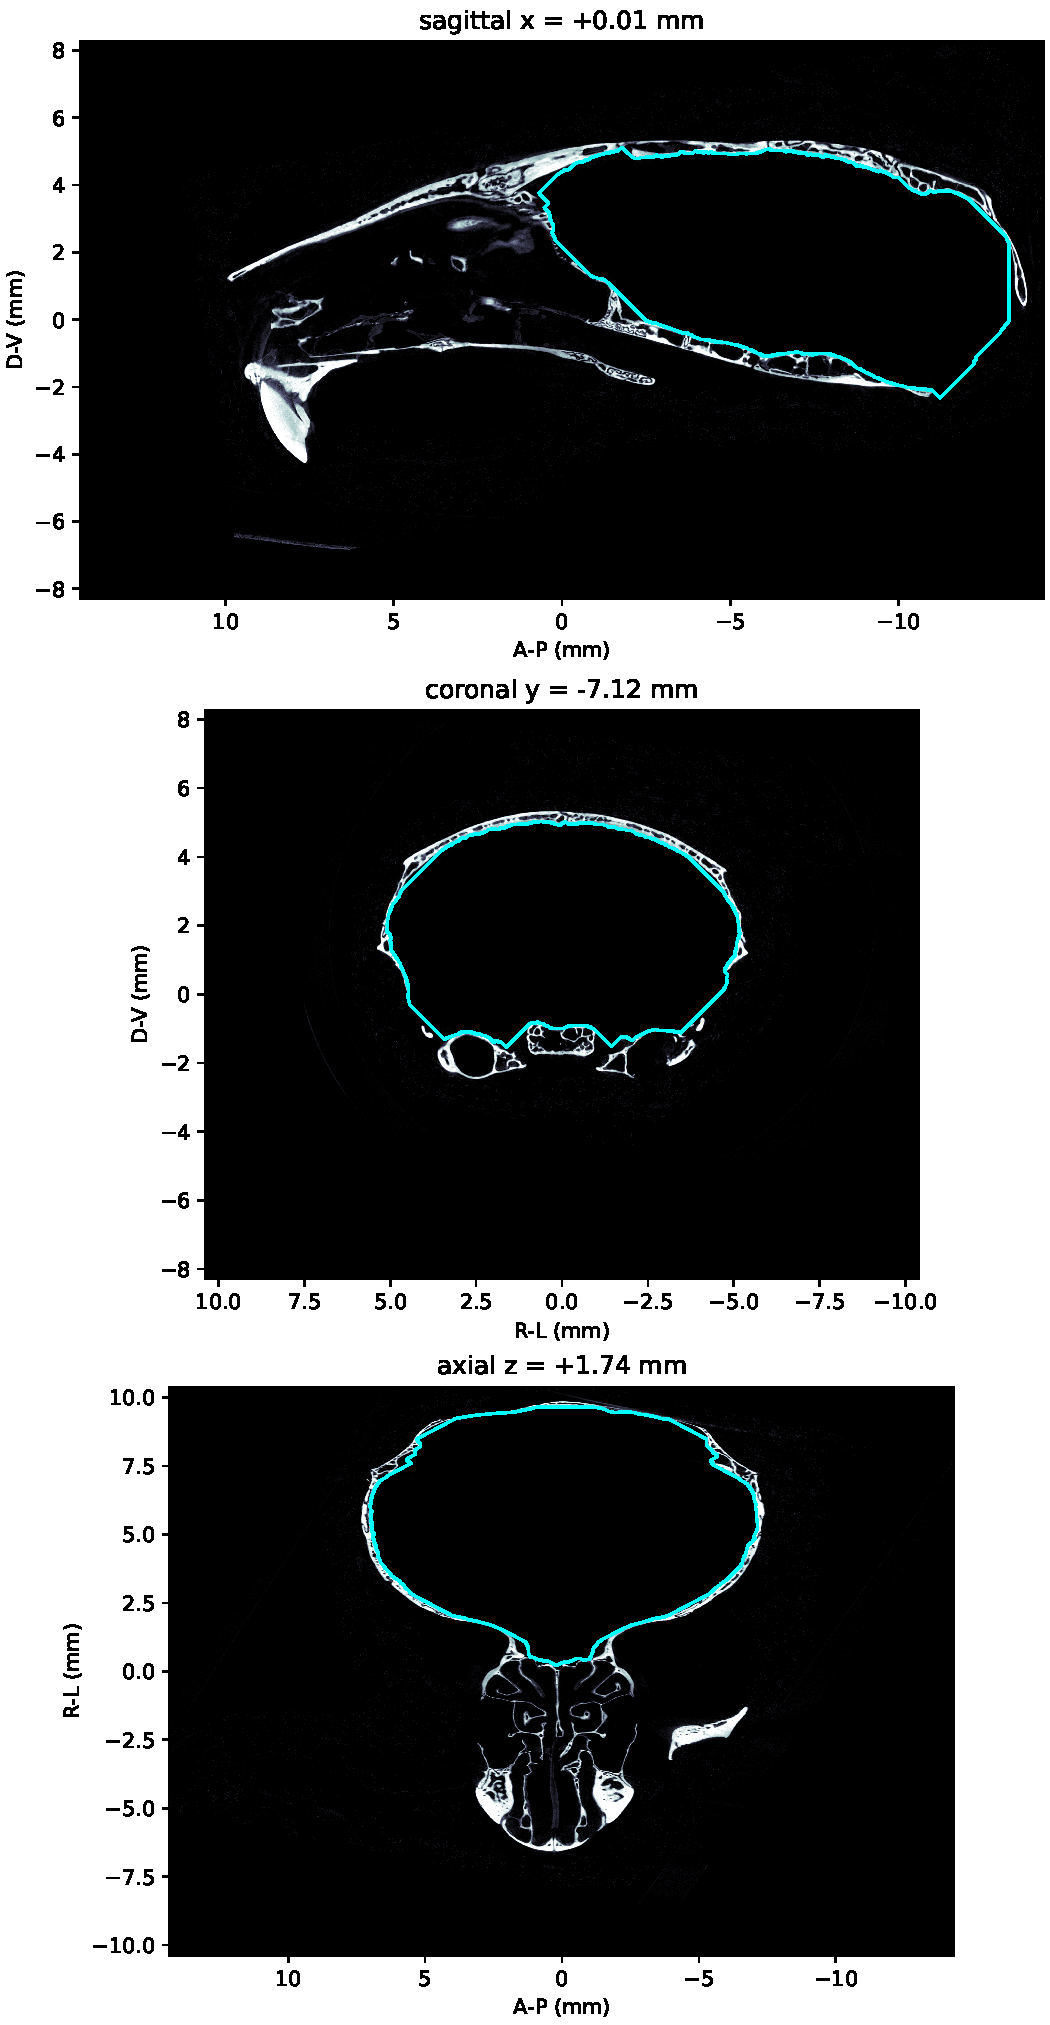
\includegraphics[width=0.85\textwidth,keepaspectratio]{cavity_qc.pdf}
\caption{Endocranial cavity overlaid on the Maga 4K skull at native
         6.127\,$\mu$m resolution. Sagittal, coronal, and axial
         sections (top to bottom) through the cavity centroid (in
         world coords) show the extracted contour (cyan) over the
         source intensity volume (greyscale). The cavity mask is
         extracted at 24.5\,$\mu$m (factor-4 block-max decimation
         of the aligned native) and is the moving image for the SyN
         registration of \S\ref{sec:registration}; each panel is
         rendered at 1200\,dpi. The 25\,$\mu$m cache inherits the
         native's world frame by construction (block-max of the
         aligned native rather than independent alignment of a raw
         coarse cache), so native and cavity grids superimpose at
         the correct world coordinate independently of resolution.}
\label{fig:cavity-qc}
\end{figure}

% =============================================================================
\section{Allen CCFv3 to cavity registration}
\label{sec:registration}

We register the extracted Maga endocranial cavity to the Allen
CCFv3 brain template using ANTs SyN, exactly mirroring the DigiMouse
pipeline
(legacy \texttt{mouse\_therapy/registration/\allowbreak register\_cavity\_to\_allen.py};
not in TUBA)
with Maga-specific inputs and outputs. The Maga-version registration
(\texttt{tuba.species.mouse.\allowbreak register\_to\_atlas} and
\texttt{warp\_atlas\_into\_maga})
reads
\texttt{maga\_cranial\_cavity.nii.gz} as the moving image, the
binarised Allen brain mask (template intensity $> 5$\,\% of max) as
the fixed image, and writes the forward/inverse transforms to
\texttt{maga\_cavity\_to\_allen\_syn\_*.txt}. The cavity moving image
and the Allen brain mask fixed image now share a working resolution of
$\sim$25\,$\mu$m (24.5\,$\mu$m for the Maga cache, 25\,$\mu$m for the
Allen brain mask): the grids match within 2\,\% in voxel pitch and the
cavity has $\sim$500 times more support voxels than the 200\,$\mu$m
mask used in earlier drafts. Affine initialisation converges quickly
and the SyN-stage cost is dominated by the residual non-linear
deformation; total SyN wall time on a single Threadripper core remains
under 2\,min.

For the \emph{warped} Allen products we then apply the same SyN
transforms but source from the 10\,$\mu$m Allen template and annotation
(via \texttt{ants.apply\_transforms}). Because ANTs transforms are
stored in world coordinates, the 25\,$\mu$m-derived warp is valid for
the 10\,$\mu$m moving image; the result is a higher-detail warped
template/annotation sampled onto the Maga 25\,$\mu$m cavity grid. Running the
SyN itself at the 10\,$\mu$m fixed resolution would cost $\sim$1\,h
because the deformation field is held at the full Allen grid
(1.2\,Gvoxels $\times$ 3 components $\times$ 4\,bytes $\approx$ 14\,GB
per field); the hybrid keeps the SyN at 25\,$\mu$m and uses the 10\,$\mu$m
source only at the resampling step where it costs nothing.

After the SyN converges, the script pushes the Allen brain template
back into Maga space using a linear interpolator, and pushes the
Allen anatomical annotation volume back using a nearest-neighbour
interpolator (preserving region IDs). These two products are saved
as \texttt{allen\_template\_}\allowbreak\texttt{in\_maga.nii.gz} and
\texttt{allen\_annotation\_}\allowbreak\texttt{in\_maga.nii.gz}
respectively and are the inputs to the registration QC figure.

Fig.~\ref{fig:registration} shows the result in two columns. The left
column overlays the warped Allen template intensity (warm colour) on
the Maga skull, demonstrating that the template fills the extracted
endocranial cavity without obvious mass-effect leakage into the
turbinate region or down the foramen magnum. The right column
overlays the warped Allen \emph{annotation} (594 distinct anatomical
region IDs after restriction to the cavity bounding box) using a
saturated per-region colour palette; this gives a high-contrast
side-by-side view of how the Allen Common Coordinate Framework maps
onto the actual skull. The match of the smooth cavity contour (cyan)
to the lateral boundary of the colour-coded brain in every orthoslice
is the principal L-R / D-V sanity check: had any axis flag in
\texttt{tuba.species.mouse} been wrong, or the rigid
pre-alignment (\S\ref{sec:align}) failed, the warped atlas would
either fail to fit or would mirror across the midline. The current
result shows the atlas filling the cavity within the $\sim$25\,$\mu$m
registration tolerance, confirming that both the storage-axis flips
and the PCA-derived pre-rotation are correct.

\begin{figure}[p]
\centering

\includegraphics[width=\textwidth,keepaspectratio]{registration_qc.pdf}
\caption{Allen CCFv3 $\to$ Maga skull registration QC at native
         6.127\,$\mu$m resolution, in portrait layout. Three
         orthoslices (sagittal, coronal, axial, top to bottom) through
         the cavity centroid. \textbf{Left column}: greyscale Maga
         skull at native pixel grid with the warped Allen brain
         template intensity overlaid in warm colour. \textbf{Right
         column}: same skull background with the warped Allen
         anatomical annotation overlaid as a saturated per-region
         colour map (each Allen structure ID a distinct hue from a
         perceptually distinct palette). Cyan = endocranial cavity
         contour. Warped Allen overlays live on the 25\,$\mu$m Maga
         reference grid (with 10\,$\mu$m source detail from the
         moving template/annotation), the cavity contour on the
         24.5\,$\mu$m cache grid, and the native skull on the
         6.127\,$\mu$m grid; matplotlib places each at its own
         world-coordinate extent so the three pixel grids superimpose
         without resampling. Each panel is rendered at 1200\,dpi.}
\label{fig:registration}
\end{figure}

% =============================================================================
\section{Acoustic-property mapping}
\label{sec:acoustic-mapping}

The transcranial FDTD and angular-spectrum simulations require per-voxel
maps of sound speed $c(\mathbf{r})$, density $\rho(\mathbf{r})$, and
attenuation $\alpha(\mathbf{r})$. The DigiMouse pipeline derives these
from the uint8 mouseCT byte values via a piecewise-linear ramp defined
in legacy \texttt{mouse\_therapy/registration/\allowbreak mouse\_skull\_slab\_3d.py}
(not in TUBA): voxels below the
soft-to-bone threshold (byte 210) are assigned water-equivalent
properties ($c=1540$\,m/s, $\rho=1000$\,kg/m$^3$), while bone voxels
ramp linearly to cortical-bone values ($c=2900$\,m/s,
$\rho=1900$\,kg/m$^3$) at byte 255. A skull-shell constraint (maximum
1.2\,mm distance from the outer head surface) is imposed in order to
suppress a measurement artefact specific to the DigiMouse atlas: the
cranial-cavity bytes saturate at 255 throughout the brain (likely a
fixation/contrast artefact, not actual cortical bone), so the same
threshold without a distance constraint would classify the entire
endocranium as bone.

The Maga 4K scan presents a different mapping problem. The dry skull
contains air in the endocranial cavity and the published reconstruction
log records no hydroxyapatite step-wedge phantom or HU calibration
(Table~\ref{tab:scan-params}, Table~\ref{tab:source-compare}), so the
uint16 NRecon counts cannot be bound to absolute mineral-density units.
We adapt the DigiMouse mapping with three changes, implemented in
\texttt{tuba.species.mouse.\allowbreak load\_slab}. The Maga slab
loader exposes the same
\texttt{load\_slab(apex\_world\_mm, beam\_3d, slab\_size\_m, dx\_target\_m)}
signature as \texttt{tuba.species.\{macaque,human\}.load\_slab} and as
the legacy DigiMouse \texttt{load\_mouse\_skull\_slab\_3d}, so any
FDTD or angular-spectrum driver wired against one species runs on the
other unchanged (only the species module changes).

\paragraph{Mapping function.} The histogram of \S\ref{sec:cavity},
Fig.~\ref{fig:histogram}, resolves three populations: air ($<100$
uint16), mounting material at 4--8\,k\,cts, and cortical bone with a
mode at $\sim$25\,k\,cts and a tail extending to 40\,k\,cts. We anchor the acoustic
ramp on two histogram-derived intensities, both already used by the
cavity extractor of \S\ref{sec:cavity}:
\begin{itemize}[leftmargin=*]
\item $I_{\mathrm{low}} = \texttt{BONE\_LOW} = 5000$: voxels at or below
      this are water/soft-tissue ($c=1540$\,m/s, $\rho=1000$\,kg/m$^3$).
\item $I_{\mathrm{high}} = 25\,000$ (cortical-bone histogram mode):
      voxels at or above this saturate at cortical-bone values
      ($c=2900$\,m/s, $\rho=1900$\,kg/m$^3$).
\end{itemize}
Between $I_{\mathrm{low}}$ and $I_{\mathrm{high}}$ the acoustic
properties ramp linearly. Choosing the histogram \emph{mode} rather than
the global maximum as the cortical-bone anchor makes the mapping robust
to the detector- and reconstruction-dependent absolute NRecon scale: the
literature endpoint ($\rho=1900$\,kg/m$^3$, $c=2900$\,m/s) is bound to
the cortical peak \emph{of this scan} rather than to a numerically
arbitrary saturation value. This sacrifices absolute calibration -- a
hydroxyapatite phantom would let us bind a specific NRecon count to a
specific HU and thence to a calibrated density -- but it gives a
deterministic, reproducible mapping with no free parameters once
$I_{\mathrm{low}}$ and $I_{\mathrm{high}}$ are fixed by the histogram.

\paragraph{Cavity infill and exterior masking.} The endocranial cavity
extracted in \S\ref{sec:cavity} contains air in the source scan but is
populated with brain-parenchymal acoustic properties for the simulation
($c=1540$\,m/s, $\rho=1040$\,kg/m$^3$, with attenuation as below).
Outside the bone shell, the 4--8\,k\,cts mounting-material plateau is below
$I_{\mathrm{low}}$ and is therefore mapped to water -- the matched-fluid
coupling assumption used by the DigiMouse pipeline. No shell-distance
constraint is required: the Maga endocranial cavity contains air, not
saturated tissue, so the bone shell and the dry-skull cavity are
already well-separated by the intensity threshold. The cavity mask from
\S\ref{sec:cavity} is used only to identify the parenchymal-fill region;
voxels classified as bone retain their intensity-derived $(c, \rho)$
values even when they fall inside the cavity bounding box.

Fig.~\ref{fig:acoustic-mapping} visualises the mapping at the
200\,$\mu$m grid: the left panel overlays the $c$ and $\rho$ ramps on
the log-binned intensity histogram of the aligned cache, and the
centre/right panels show coronal slices of the resulting $c$- and
$\rho$-maps with the cavity infill applied. The bone shell appears as
a saturated ring at $(c, \rho)=(2900, 1900)$, the parenchymal-fill
region as a uniform interior at $(1540, 1040)$, and the
mounting-material plateau outside the bone correctly maps to water.

\begin{figure}[H]
\centering
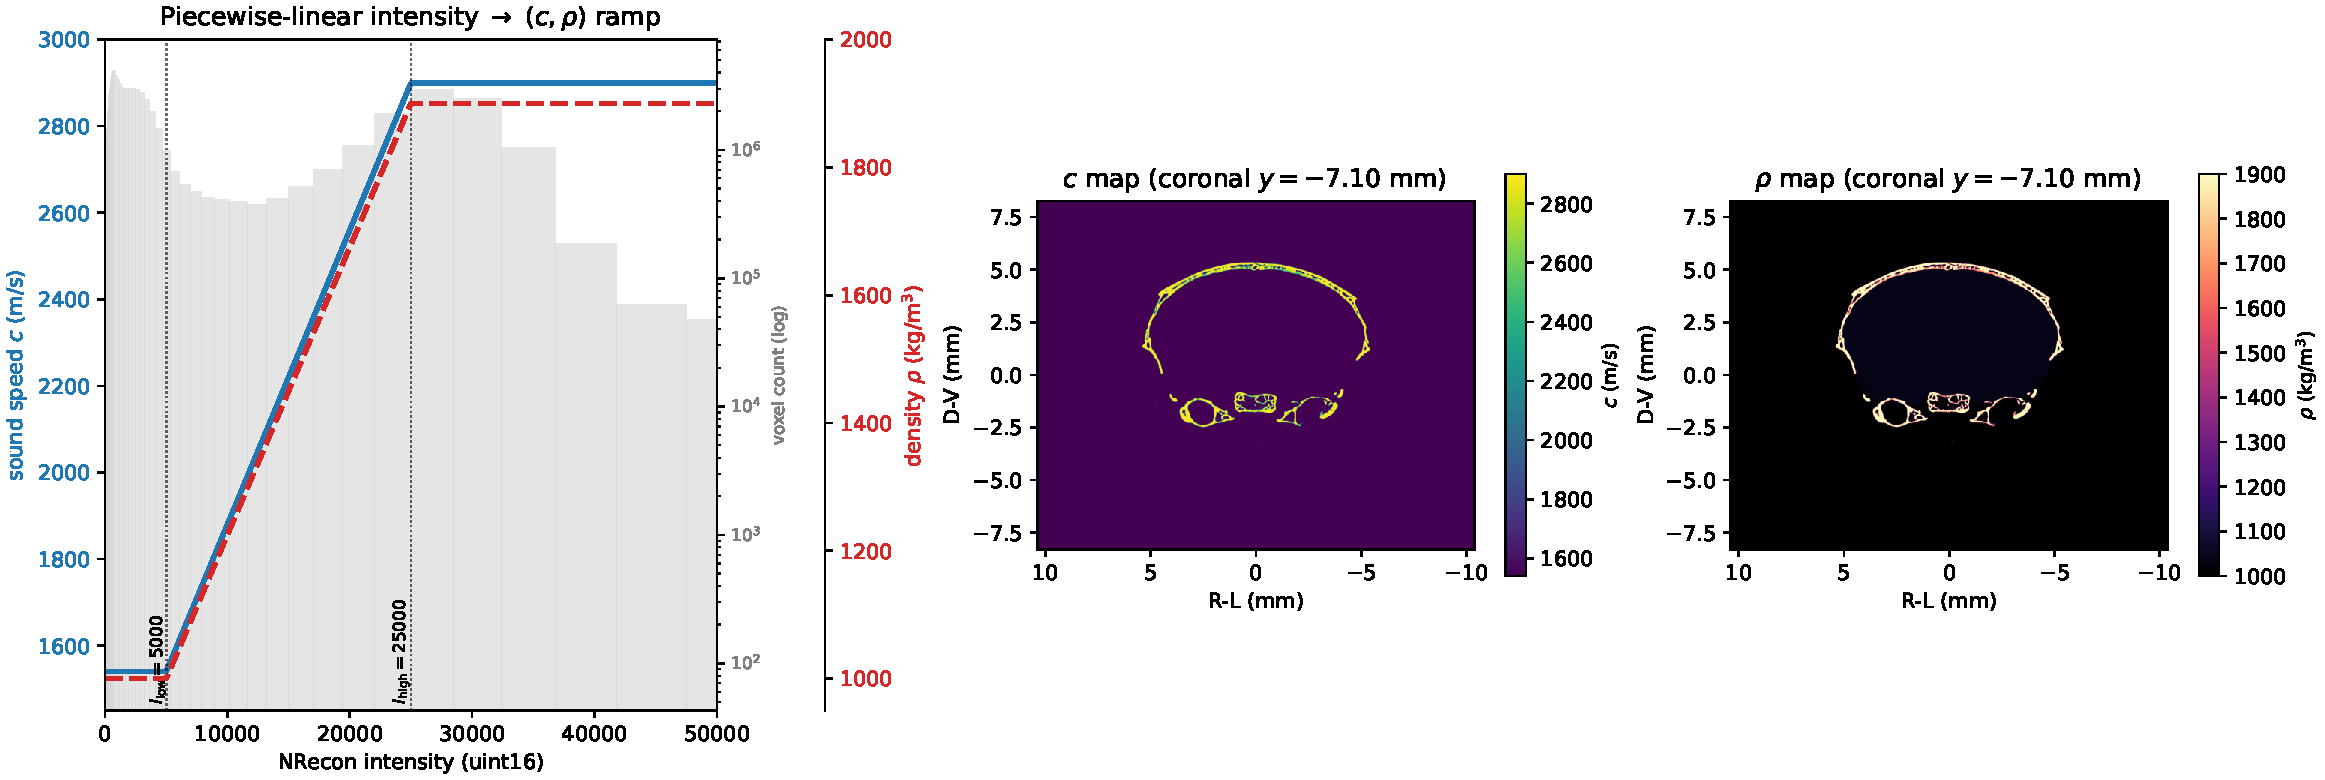
\includegraphics[width=\textwidth,keepaspectratio]{acoustic_mapping_qc.pdf}
\caption{Acoustic-property mapping for the Maga 4K skull (\S\ref{sec:acoustic-mapping}).
         \textbf{Left}: piecewise-linear intensity~$\to$~$(c, \rho)$ ramp
         (blue: $c$, m/s; red dashed: $\rho$, kg/m$^3$) overlaid on the
         log-binned intensity histogram of the aligned 200\,$\mu$m
         cache (light grey, secondary y-axis). The $I_{\mathrm{low}}=5000$
         and $I_{\mathrm{high}}=25\,000$ anchors are marked with
         dotted vertical lines. \textbf{Centre}: $c$ map (m/s) on a
         coronal slice through the cavity centroid, with the cavity
         parenchymal-fill applied. \textbf{Right}: $\rho$ map
         (kg/m$^3$) on the same slice. Bone-classified voxels saturate
         at $(2900, 1900)$; the cavity infill is $(1540, 1040)$; the
         exterior and mounting-material region maps to water
         $(1540, 1000)$.}
\label{fig:acoustic-mapping}
\end{figure}

\paragraph{Attenuation.} We adopt the frequency-power-law model and
coefficients of the DigiMouse pipeline unchanged:
$\alpha_{\mathrm{bone}} = 8$\,dB\,cm$^{-1}$\,MHz$^{-1}$,
$\alpha_{\mathrm{brain}} = \alpha_{\mathrm{tissue}} = 0.5$\,dB\,cm$^{-1}$\,MHz$^{-1}$
at 15\,MHz, with linear frequency dependence ($\alpha \propto f$).
Validation against the Maga 4K skull would require a complementary
transmission measurement at 15\,MHz that is not part of the source data
release; this is left to future work. The simulation results in
\S\ref{sec:comparison} should therefore be read as indicative of the
relative effect of replacing the DigiMouse skull volume with the Maga
4K skull volume, holding all other acoustic-property choices fixed.

% =============================================================================
\section{Focal-prediction comparison}
\label{sec:comparison}

The forward simulation that produced
Table~\ref{tab:focal-comparison} and Fig.~\ref{fig:focal-comparison}
ran the same skull-agnostic driver against both species; the legacy
\texttt{mouse\_therapy/run\_mouse\_cc.py} dispatched on the slab-loader
/ placement-helper pair for each species (DigiMouse via
\texttt{mouse\_skull\_slab\_3d} / \texttt{mouse\_placement}, Maga 4K
via the equivalents now consolidated in \texttt{tuba.species.mouse}),
without otherwise changing the bowl geometry, drive level, target
convention, FDTD/angular-spectrum grid, attenuation model, or
post-processing. Both pipelines focus a 10\,mm-aperture / 10\,mm-ROC
($f/1$) bowl at $f_0=15$\,MHz on the cranial-cavity centroid, with a
3-cycle tone burst and a drive level calibrated post-hoc so that the
free-field-equivalent peak-negative pressure (PNP) equals the
$\mathrm{MI}=1.9$ target ($7.359$\,MPa). Any difference in the
predicted focal field is therefore attributable to the skull volume.

\paragraph{Simulation parameters.} The shared grid is
$409\times 409$ lateral $\times 413$ time samples at
$\Delta x = \lambda/3.5 = 29.3$\,$\mu$m,
$\Delta t = 3.81$\,ns, over a $12\times 12\times 15$\,mm domain. The
beam-aligned skull slab is sampled at the same $\Delta x$, with the
DigiMouse loader sampling the 100\,$\mu$m mouseCT cache and the Maga
loader sampling the 25\,$\mu$m aligned-native cache. The DigiMouse
sampler restricts bone classification to a 1.2\,mm shell of the outer
head surface (\S\ref{sec:acoustic-mapping}), whereas the Maga sampler
classifies bone by intensity alone over the full slab.

\paragraph{Results.}
Table~\ref{tab:focal-comparison} reports the focal-spot metrics
extracted from both runs. Fig.~\ref{fig:focal-comparison} shows the
corresponding skull cross-sections, $|p|$-fields (peak-normalised in
dB), and on-axis / lateral pressure profiles through the focal peak.

\begin{table}[H]
\centering
\caption{Focal-spot metrics at $f_0=15$\,MHz for the DigiMouse atlas
         versus the Maga 4K dry skull, with identical bowl, drive
         calibration, grid, and target. Peak pressure is the maximum
         of $|\mathrm{PNP}|$ over the post-source half of the domain;
         focal position is the $|\mathrm{PNP}|$-argmax coordinate;
         lateral / axial FWHM are full-width at half-pressure-maximum
         through that argmax voxel along the corresponding axis.
         Relative skull transmission is the ratio of unit-drive
         transcranial focal pressures, in dB.}
\label{tab:focal-comparison}
\begin{tabular}{lrrr}
\hline
Metric & DigiMouse & Maga 4K & $\Delta$ \\
\hline
Unit-drive focal $|p|$ (Pa) & 5.77 & 5.37 & $-0.39$ \\
Drive amplitude $p_0$ for MI = 1.9 (MPa) & 1.27 & 1.36 & $+0.09$ \\
Calibrated focal $|p|$ (MPa) & 7.32 & 7.31 & $-0.01$ \\
Focal $x$ (mm) & $+0.00$ & $+0.00$ & $\pm 0.00$ \\
Focal $y$ (mm) & $+0.00$ & $+0.00$ & $\pm 0.00$ \\
Focal $z$ (mm)\textsuperscript{\dag} & 10.21 & 9.83 & $-0.38$ \\
FWHM lateral $x$ (mm) & 0.205 & 0.177 & $-0.028$ \\
FWHM lateral $y$ (mm) & 0.219 & 0.211 & $-0.008$ \\
FWHM axial $z$ (mm) & 1.457 & 1.356 & $-0.101$ \\
\hline
\multicolumn{4}{l}{Relative skull transmission (Maga $-$ DigiMouse):
                    $-0.62$\,dB at unit drive} \\
\hline
\multicolumn{4}{l}{\textsuperscript{\dag}Geometric focus at
                    $z = 10.0$\,mm; DigiMouse $+0.21$, Maga $-0.17$\,mm
                    (both $\le 0.25$\,mm).} \\
\end{tabular}
\end{table}

\begin{figure}[H]
\centering
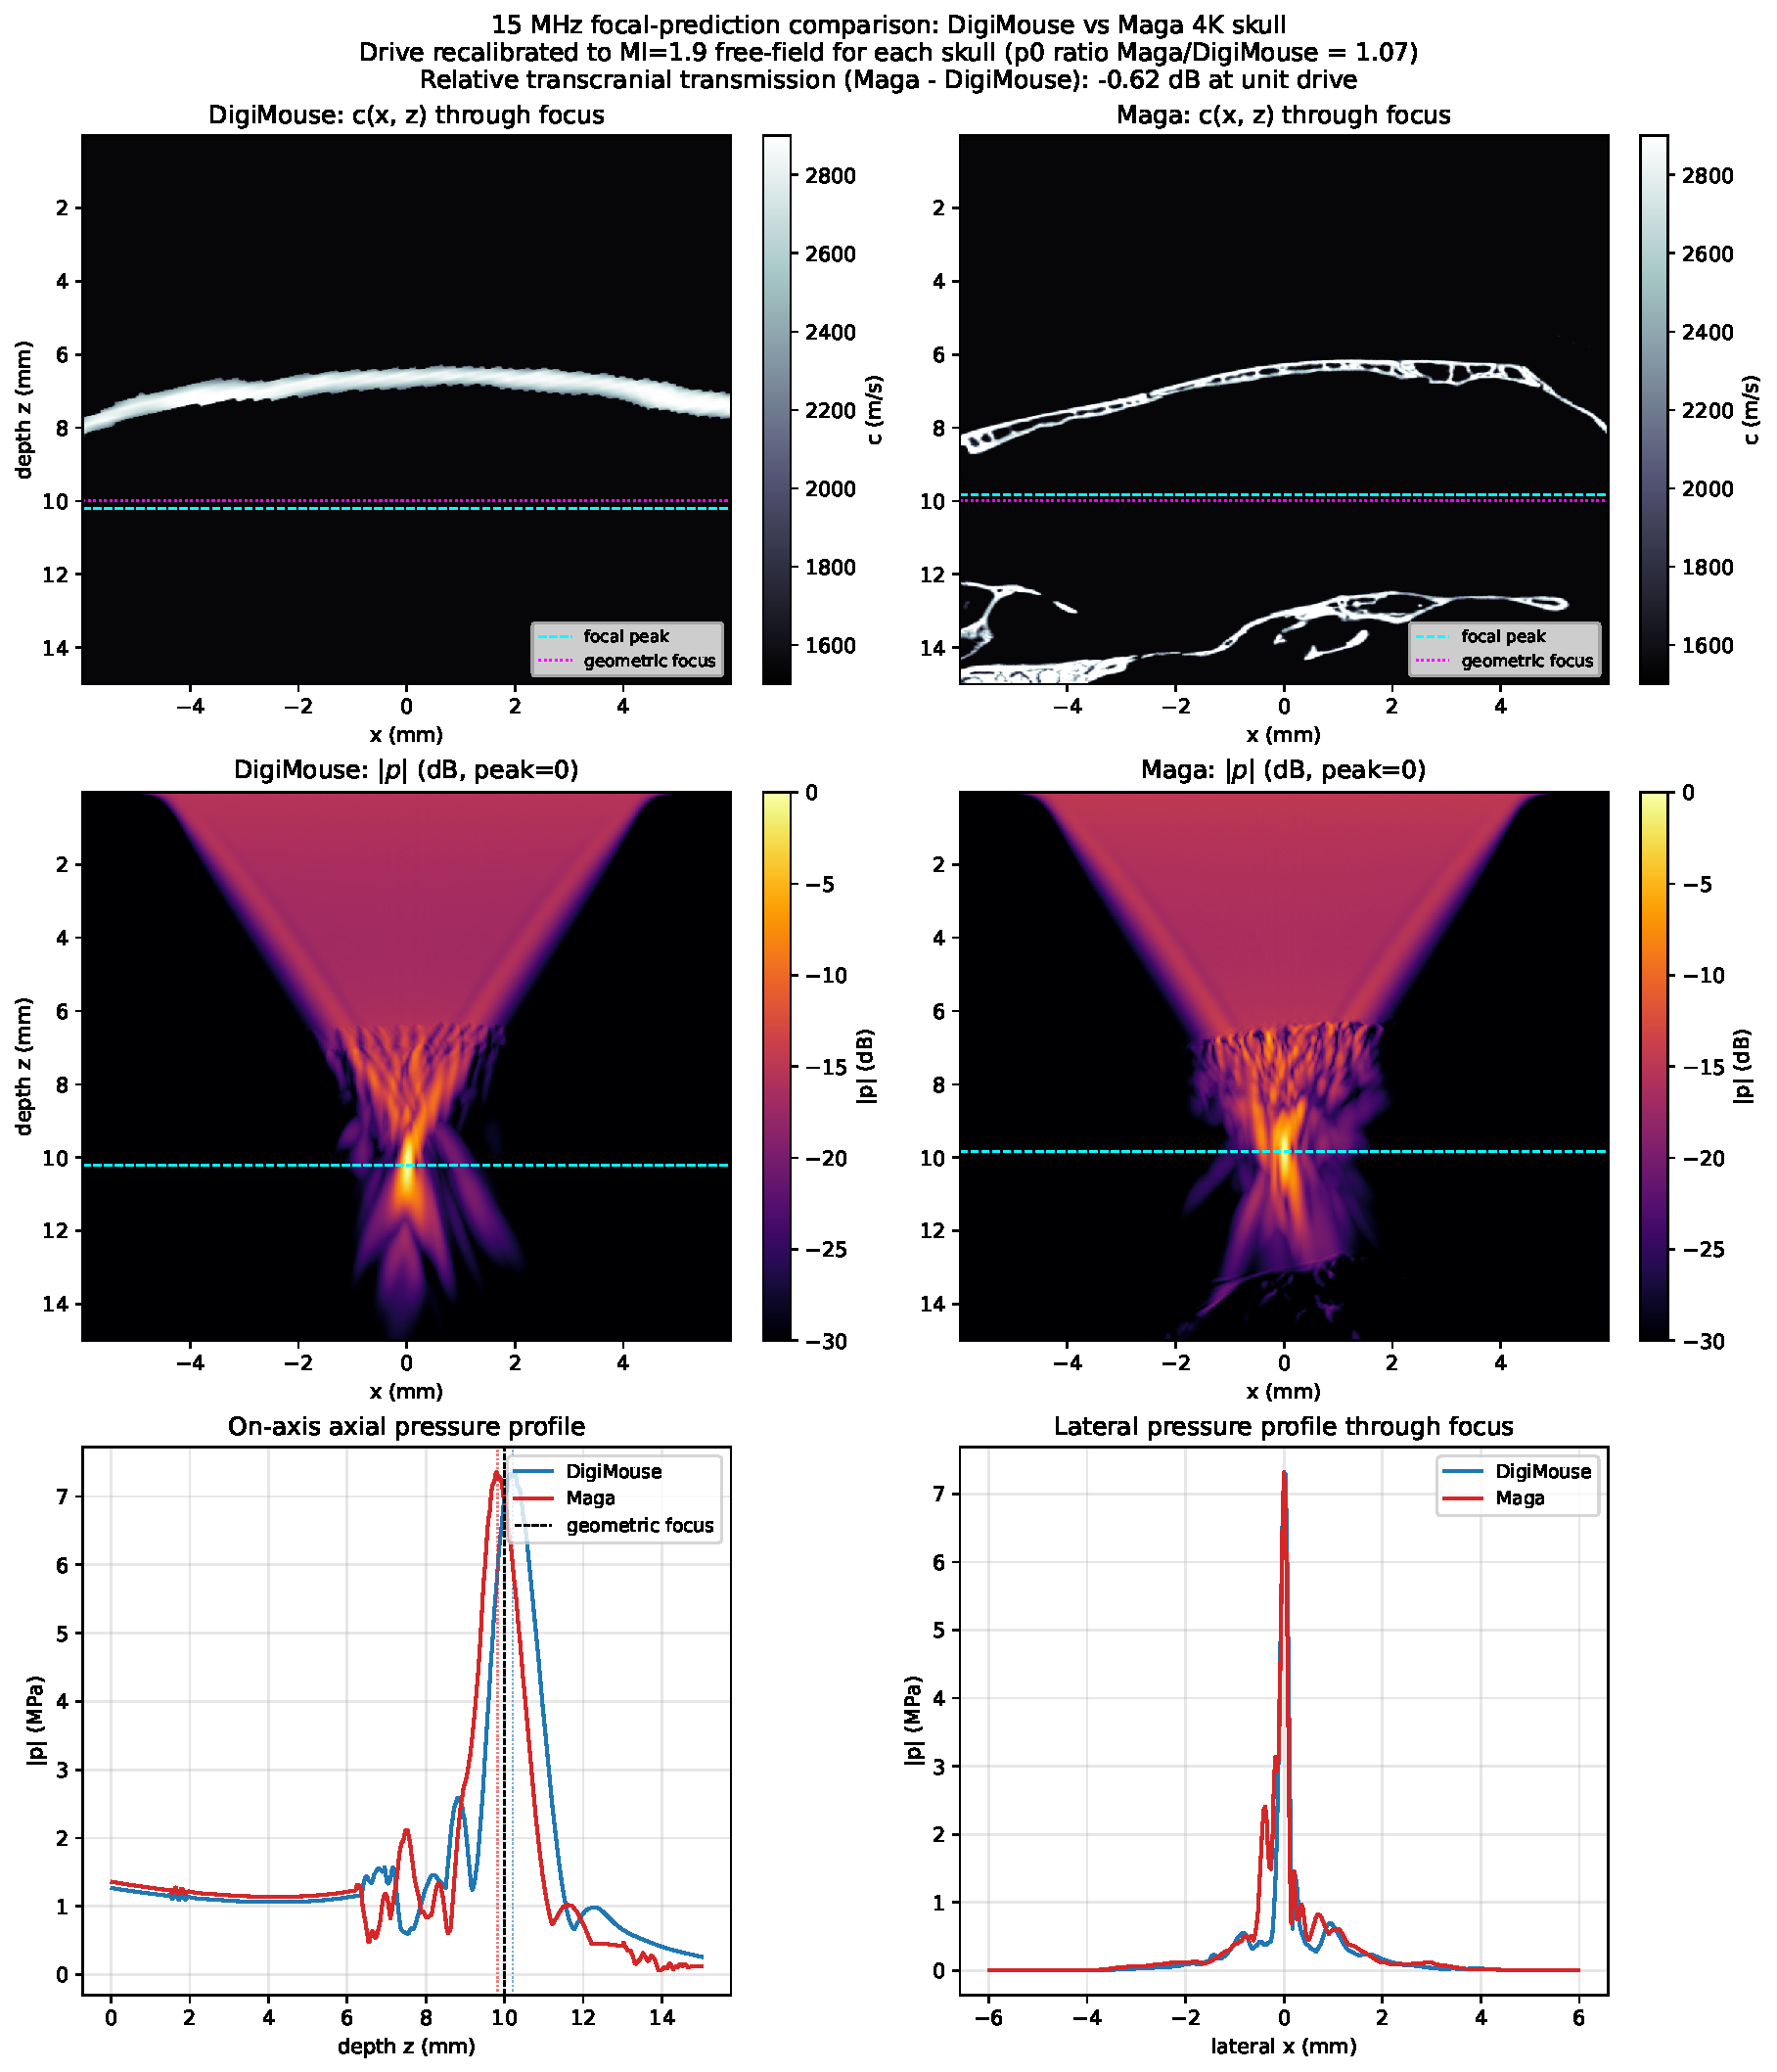
\includegraphics[width=\textwidth,keepaspectratio]{focal_comparison.pdf}
\caption{15\,MHz focal-prediction comparison (\S\ref{sec:comparison}).
         \textbf{Top}: sound-speed cross-section through the focal
         peak. The DigiMouse panel shows the 1.2\,mm shell-restricted
         bone classification adopted to suppress the saturated-tissue
         artefact (\S\ref{sec:acoustic-mapping}); the Maga panel
         shows the intensity-classified cortical bone over the full
         slab depth, including the rostral snout fragment caught by
         the $20^{\circ}$ sagittal-plane ($y$-$z$) tilt at
         $z\sim 12$--14\,mm.
         \textbf{Centre}: $|p|$ in dB (peak-normalised) on the same
         coronal slice; cyan dashed line marks the
         transcranial focal $z$. \textbf{Bottom}: on-axis axial and
         lateral pressure profiles through the
         $|\mathrm{PNP}|$-argmax voxel for the calibrated drives
         (DigiMouse: $p_0 = 1.27$\,MPa, Maga: $p_0 = 1.36$\,MPa).}
\label{fig:focal-comparison}
\end{figure}

\paragraph{Anatomical context.} The beam-aligned slab grid used by
the angular-spectrum solver has its own coordinate frame (lateral /
elevation / depth, aligned to the bowl axis); to read off which Allen
CCFv3 structures the focal field intersects, we resample the
intensity volume from the slab grid back into the Allen frame: each
voxel of the Maga 25\,$\mu$m
aligned cache is projected onto the slab basis
$(\mathbf{t}_1, \mathbf{t}_2, \mathbf{beam})$ defined by the
placement, the intensity is sampled by linear interpolation, and the
resulting Maga-frame volume is then warped through the SyN forward
transforms of \S\ref{sec:registration} into the Allen 25\,$\mu$m grid.
Fig.~\ref{fig:intensity-on-allen} shows three orthogonal Allen slices
through the focal peak with the warped intensity overlaid, both on
the anatomical template (top row) and on the colour-coded structure
annotation (bottom row). The focal peak lands at Allen world
$(+0.06, -0.76, +0.24)$\,mm -- essentially at Bregma in the midline,
within the corpus-callosum / thalamus boundary region targeted by the
$f/1$ bowl placement.

\begin{figure}[H]
\centering
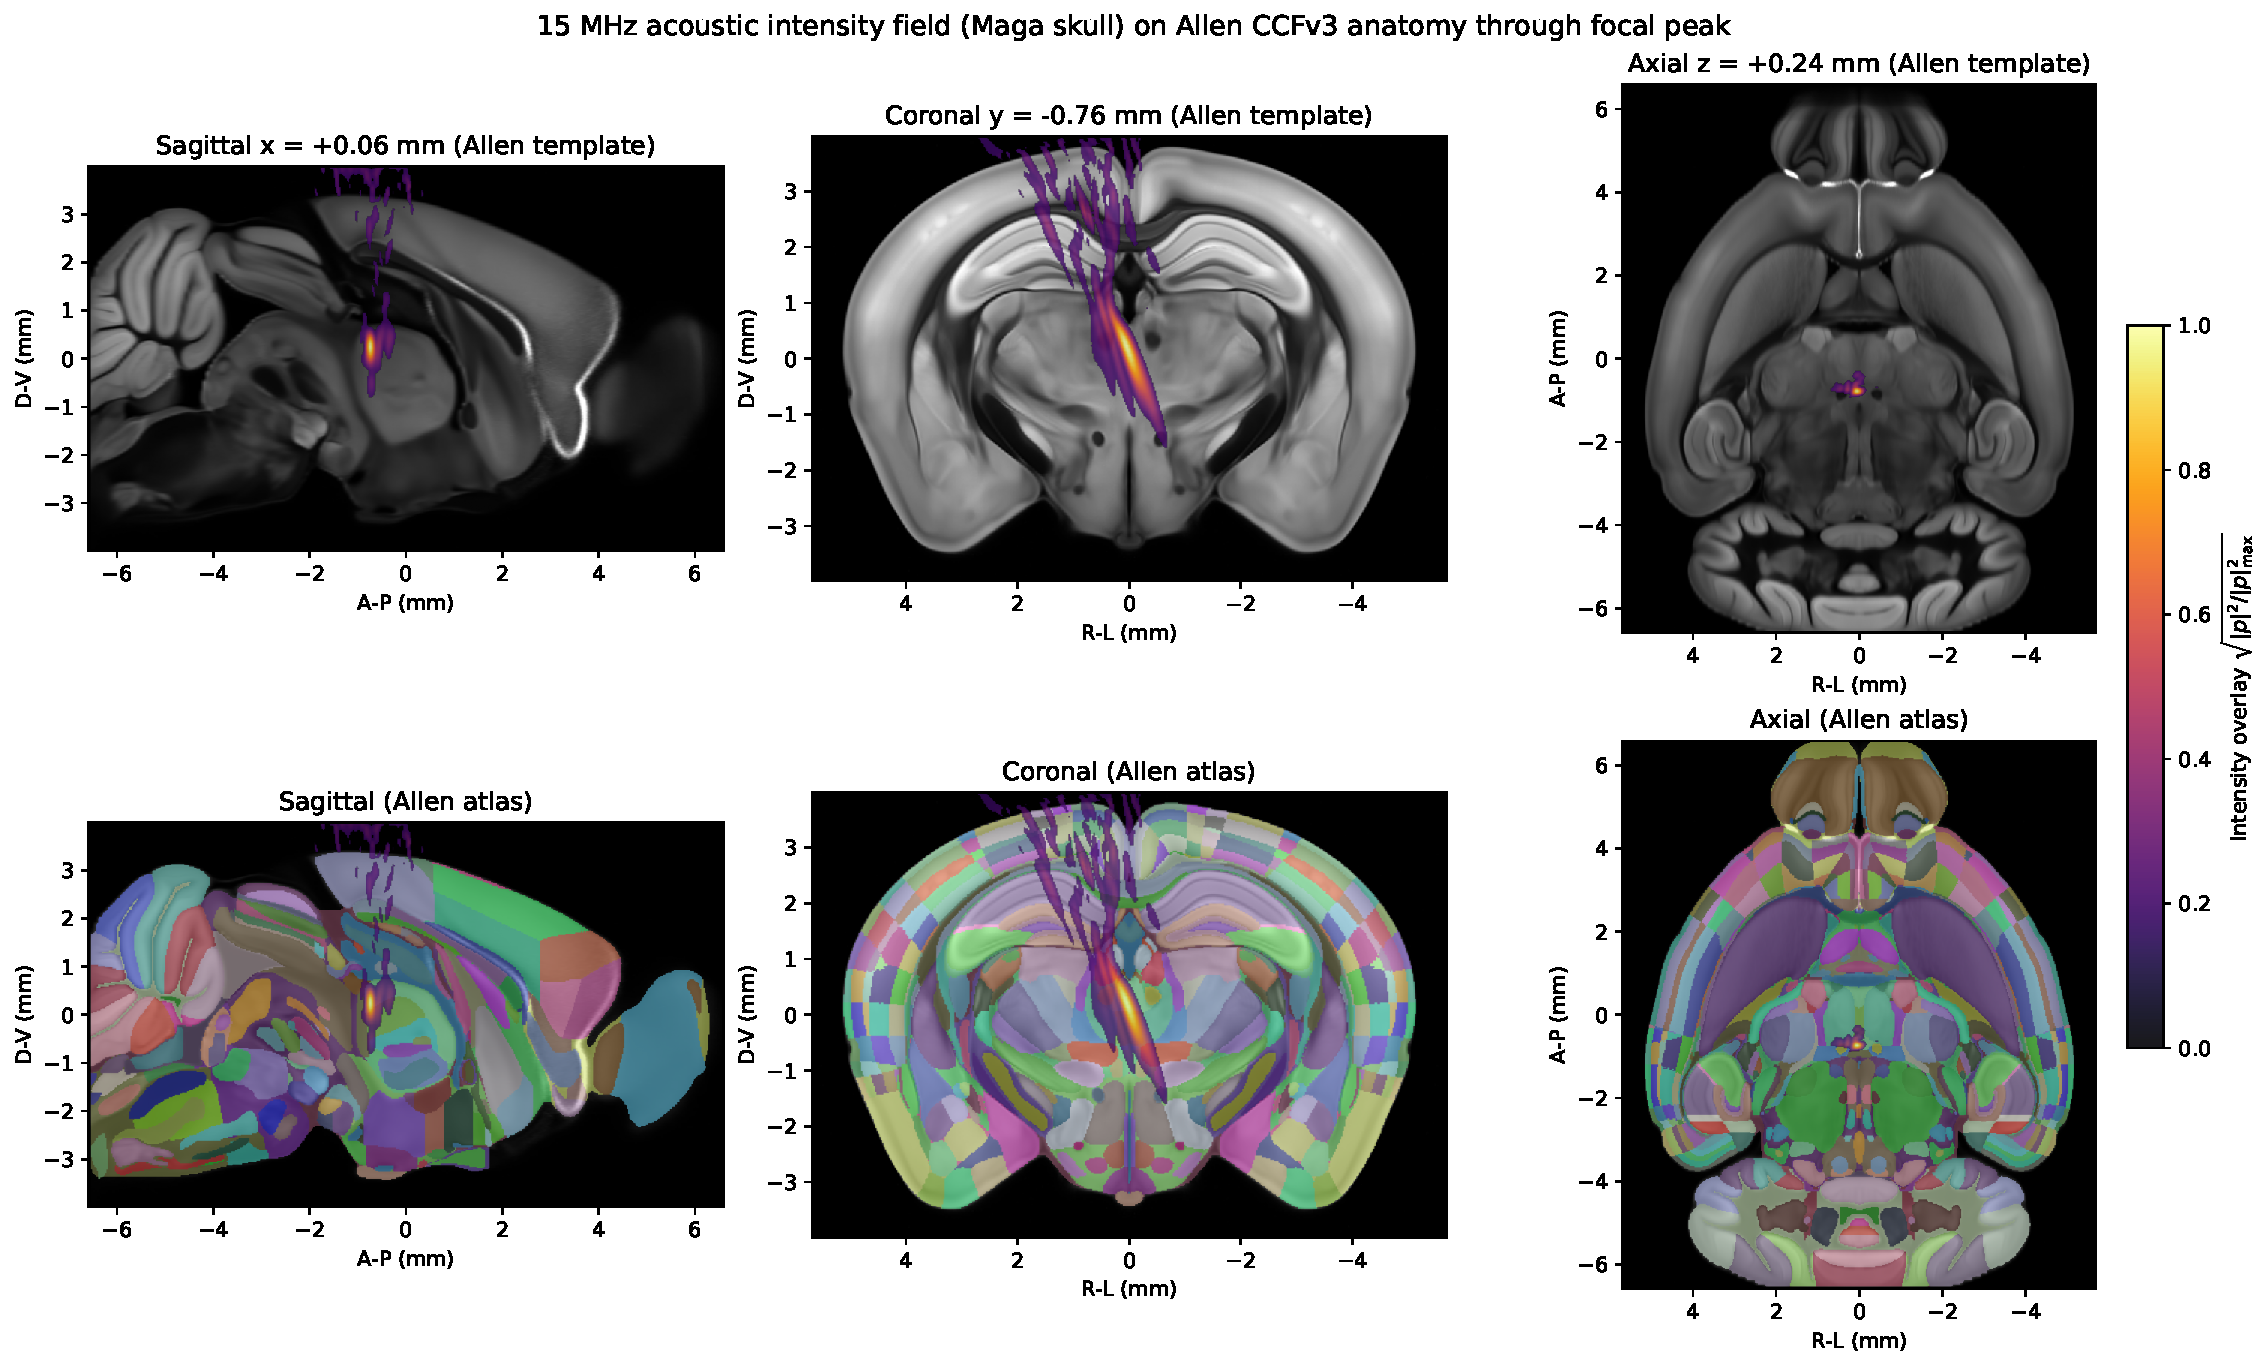
\includegraphics[width=\textwidth,keepaspectratio]{intensity_on_allen.pdf}
\caption{15\,MHz acoustic intensity field from the Maga skull
         simulation, resampled into the Allen CCFv3 frame and overlaid
         on Allen anatomical slices through the focal peak
         (\S\ref{sec:comparison}). Overlay colour:
         $\sqrt{|p|^2 / |p|^2_{\max}}$ (i.e. pressure amplitude
         normalised to the focal peak); voxels below $-15$\,dB
         pressure are made transparent so the underlying anatomy
         remains visible. \textbf{Top}: Allen 25\,$\mu$m anatomical
         template. \textbf{Bottom}: Allen CCFv3 region annotation
         (RGBA per structure id). The intensity tail extending
         dorsally and slightly anterior reflects the bowl axis after
         the $20^{\circ}$ sagittal-plane tilt
         (\texttt{MOUSE\_CC\_TILT\_DEG}); the focal spot sits in the
         midline at Bregma.}
\label{fig:intensity-on-allen}
\end{figure}

\paragraph{Interpretation.}
The two skull volumes produce focal predictions that agree to within
sub-grid precision once the drive is recalibrated. The $-0.62$\,dB
($\equiv 7\%$ in pressure) number quoted in
Table~\ref{tab:focal-comparison} is the ratio of unit-drive
transcranial focal pressures (Maga over DigiMouse) in dB;
equivalently, the difference of per-skull transmission losses
measured against a common homogeneous free-field reference
(Maga 14.61\,dB vs.\ DigiMouse 15.22\,dB total loss at the
$f_0 = 15$\,MHz, $f/1$ geometry of this study). With the bowl,
drive, grid, and target held fixed, both expressions evaluate to
the same number. In practical terms, the Maga model requires
$\sim 7\%$ more electrical drive to hit the same intracranial
pressure target; the focal-spot lateral FWHM is slightly tighter
($-0.028$\,mm in $x$, $-0.008$\,mm in $y$) and the axial FWHM
slightly shorter ($-0.101$\,mm), but both differences are at or below the
$\Delta x = 29.3$\,$\mu$m sub-grid level for lateral and at the
$\sim 5\%$ level for axial. The focal $z$ depth shift of $-0.38$\,mm
($\sim\!\!13\Delta x$) is well within the 0.68\,mm focal-spot
axial half-width, consistent with a small refractive bias from the
curved cortical-bone interface that the Maga slab captures and the
DigiMouse shell flattens out.

\paragraph{What this does not measure.} The comparison holds the
acoustic-property mapping fixed (the piecewise-linear ramp of
\S\ref{sec:acoustic-mapping}), the attenuation coefficients fixed
($\alpha_{\mathrm{bone}} = 8$\,dB\,cm$^{-1}$\,MHz$^{-1}$,
$\alpha_{\mathrm{tissue}} = 0.5$\,dB\,cm$^{-1}$\,MHz$^{-1}$ at
15\,MHz), and the target position fixed (cavity centroid in the
respective frame). It therefore does not isolate the effect of the
ramp endpoints, the absolute attenuation calibration, or anatomical
variability between specimens. A transmission measurement at 15\,MHz
on the Maga sample, or on a Maga-style 4K micro-CT of a different
mouse, would be required to anchor the absolute drive prediction; the
present numbers should be read as the relative effect of substituting
the Maga skull volume for the DigiMouse skull volume at fixed
acoustic-property choices.

% =============================================================================

% =============================================================================
\section{Extension to non-human primates}
\label{sec:nhp}

The pipeline assembled in
\S\S\ref{sec:source}--\ref{sec:comparison} is species-agnostic in
structure but species-specific in numerical parameters (voxel size,
frequency, attenuation coefficients, cavity-extractor thresholds and
morphological-closing radius). This section sketches the parameters
and decision points required to port the same pipeline to a
non-human-primate (NHP) skull, motivated by the same therapeutic
question -- how does substituting a high-quality species-specific
microCT skull for a generic atlas-derived skull change the
focal-prediction accuracy of the transcranial FDTD /
angular-spectrum simulation.

\subsection*{Open decisions}

Four parameter choices must be settled before any code is written.

\paragraph{Species and skull microCT source.} Rhesus macaque
(\emph{Macaca mulatta}) is the obvious default given the breadth of
clinical and pre-clinical FUS work in that species, but the limiting
factor is the spatial resolution of available microCT data. The
mouse case used 6.127\,$\mu$m isotropic voxels from a dry-skull
sample (\S\ref{sec:source}); the equivalent quality for NHP
would be a dry-skull or fixed-specimen scan on a microCT (not a
clinical CT, which is typically $\ge 0.5$\,mm). Candidate sources to
survey include (i)~dry-skull microCT collections from museum or
osteology archives (e.g.\ \texttt{MorphoSource}, Smithsonian
collections), (ii)~the PRIME-DE consortium structural data (although
its modality is MRI, not CT), (iii)~published lab-collected microCTs
attached to FUS or biomechanics papers, and (iv)~the synthetic CT
component of the NIMH Macaque Template (NMT) atlas, which is
MRI-derived rather than CT-acquired but offers a usable shell at
known coordinates. Cynomolgus, baboon, and marmoset are alternatives
if a higher-resolution scan exists for those species. The selection
criterion is the same as for the mouse case: highest isotropic
voxel size, dry-skull preferred to avoid soft-tissue contrast
artefacts, open or otherwise lab-accessible licensing.

\paragraph{Brain atlas.} The mouse case used Allen CCFv3 at
10 / 25\,$\mu$m for both anatomical template and structure
annotations (\S\ref{sec:allen}, \S\ref{sec:registration}). For
macaque, candidate atlases include the NIMH Macaque Template (NMT
v2.0; T1-derived template plus CHARM cortical / SARM subcortical
parcellations at $\sim 0.25$\,mm), the D99 atlas (Saleem-Logothetis;
detailed subcortical parcellation), INIA19, and the MEBRAINS
template. For marmoset, the Brain/MINDS or NIH marmoset atlases
are the obvious choices. The selection criterion is again
resolution + parcellation richness, with a preference for atlases
that ship a structural-MRI template and a label volume on the same
grid (so ANTs SyN can register the template-to-cavity by intensity
matching and the warped annotation can be reused for target ID
extraction).

\paragraph{Anatomical target.} The mouse case targeted the
cranial-cavity centroid as a proxy for the corpus-callosum body
(\S\ref{sec:comparison}). For NHP the clinical FUS targets are
markedly different: central / ventral intermediate (Vim) thalamus
for essential tremor, ventral capsule / ventral striatum for
treatment-resistant OCD, anterior limb of the internal capsule, or
subgenual cingulate (Cg25) for depression. The target must be a
structure with an unambiguous atlas-label id; the warped annotation
in skull space is then masked to that id to produce the centroid in
skull-frame world coordinates, identical to the procedure of
\S\ref{sec:registration}.

\paragraph{Frequency and bowl geometry.} The mouse case ran at
$f_0 = 15$\,MHz with a 10\,mm-aperture / 10\,mm-ROC ($f/1$) bowl
focused 10\,mm deep. Macaque cortical bone is 5--10\,mm thick (vs.\
$\sim 0.3$\,mm in mouse) and the target depth is 30--80\,mm from
the outer skull surface, so 15\,MHz is unusable; clinical macaque
FUS systems run at 0.22--1\,MHz. The new frequency, aperture, and
ROC must be chosen jointly to (i)~place the geometric focus at the
target depth, (ii)~keep the bowl aperture below the available cap
window, and (iii)~keep the per-screen attenuation under control
($\alpha_{\mathrm{bone}}$ at 1\,MHz is $15\times$ smaller than
at 15\,MHz, so the per-mm bone loss is comparable in dB if the
beam path lengthens proportionally).

\subsection*{Pipeline mapping}

With those four choices settled, the implementation follows the same
ten-step path as the present work, with each step's mouse-specific
numerics replaced by its NHP-scale analogue:

\begin{enumerate}[leftmargin=*]
\item Convert source microCT (TIFF stack, NRRD, or DICOM) to a RAS
      NIfTI with axis-aware orientation determination
      (\S\ref{sec:orientation}) and an intensity-histogram QC figure
      identifying the air / soft-tissue / bone modes
      (\S\ref{sec:acoustic-mapping}).
\item Implement skull-to-axes rigid pre-alignment via PCA on
      bone-thresholded points (\S\ref{sec:align}), with the bone
      centroid translated to the world origin so downstream caches
      share a common frame.
\item Build the native aligned cache plus a downsampled cache at
      the chosen atlas resolution via factor-$N$ block-max
      (\S\ref{sec:downsample}, \S\ref{sec:cavity}). The atlas
      resolution will be $\sim 250$\,$\mu$m for macaque NMT, so the
      block-max factor and the cavity-extractor closing radius scale
      accordingly.
\item Extract the endocranial cavity using morphological closing of
      the bone-low mask, connected-component selection on the
      negative space, and a caudal-foramen-magnum seal
      (\S\ref{sec:cavity}). Verify the resulting volume against
      published values for the species ($\sim 80$\,cm$^3$ for
      rhesus, vs $\sim 450$\,mm$^3$ for mouse).
\item ANTs SyN registration of the atlas template to the cavity
      (\S\ref{sec:registration}); warp the atlas annotation back into
      the skull frame using the saved forward transforms.
\item Acoustic-property mapping: piecewise-linear intensity ---
      $(c, \rho)$ ramp anchored on the bone-low threshold and the
      cortical-bone histogram mode (\S\ref{sec:acoustic-mapping}).
      Attenuation coefficients ($\alpha_{\mathrm{bone}}$,
      $\alpha_{\mathrm{tissue}}$) scale with the frequency chosen in
      the previous step.
\item Placement helper analogous to
      \texttt{tuba.species.mouse.\allowbreak place\_on\_skull}: extract
      the target centroid from the warped annotation,
      project to the closest dorsal outer-bone surface point, apply
      scalp clearance / apex-to-target geometry and an optional
      sagittal-plane tilt.
\item Forward simulation: the same driver pattern with the placement
      helper / slab loader pair swapped for the NHP versions
      (\texttt{tuba.species.macaque} or similar), and the drive
      calibration (free-field MI target $\to$ post-hoc $p_0$ rescaling)
      preserved unchanged.
\item Focal-prediction comparison against a reference skull volume
      (a coarser generic-primate skull template if available, or
      absolute numbers if not) using the same Pa / dB / MPa / FWHM /
      $z$-offset metrics as Table~\ref{tab:focal-comparison}.
\item Intensity-on-atlas visualisation: warp the simulated intensity
      volume into atlas space via the SyN forward transforms and
      overlay on anatomical + region-annotation slices through the
      focal peak (\S\ref{sec:comparison}).
\end{enumerate}

\subsection*{Lessons carried forward from the mouse case}

Three points proved decisive during the mouse migration and should
shape the NHP implementation from day one rather than being learned
the hard way.

\begin{itemize}[leftmargin=*]
\item \textbf{Work at atlas-matching resolution for the cavity
      contour.} The mouse cavity extractor at the 200\,$\mu$m ANTs
      cache produced visible staircase artefacts on native-resolution
      overlays and a ${\sim}0.4$\,mm inward boundary shift from
      block-max smearing (\S\ref{sec:cavity}). Moving to 25\,$\mu$m
      (the Allen template's grid) and replacing pure dilation with
      morphological closing removed both problems. For NHP, this
      means matching the atlas resolution ($\sim 250$\,$\mu$m for
      NMT) rather than working at a convenient coarse cache.
\item \textbf{Stop the cavity at the bone-low inner surface, not
      bone-high.} Extending the cavity to the cortical (bone-high)
      inner edge via CC-selection on
      $\sim\!\!\mathrm{closing}(\mathrm{bone\_high})$ leaked through
      sutures and thin spots and engulfed the mounting-material
      region (1963\,mm$^3$ in the mouse test run vs. the expected
      450\,mm$^3$). The bone-low surface is ${\sim}1$ cortical-bone
      thickness inside the true inner surface --- below visual scale
      and well within the SyN deformation tolerance, but topologically
      reliable. NHP cortical bone is much thicker, so this ${\sim}1$
      cortical-thickness residual gap is larger in absolute terms;
      offsetting the cavity surface outward by an estimated cortical
      thickness post-hoc may be worthwhile for visual fidelity.
\item \textbf{Coordinate-frame discipline.} The slab loader expects
      apex and beam coordinates in \emph{world-mm in the
      aligned-native frame}, not voxel-mm; mixing the two cost
      several debug cycles in the mouse case. ANTs forward transforms
      saved from \texttt{ants.registration(fixed=cavity,
      moving=atlas)} are used with
      \texttt{apply\_transforms(fixed=atlas, moving=skull\_data)} to
      warp skull-frame data into atlas space (and vice versa with the
      inverse). Drive calibration is post-hoc at $p_0 = 1$\,Pa with
      rescaling to the free-field MI target, so the relative skull
      transmission drops out of the unit-drive focal-pressure ratio
      cleanly --- this convention should carry over unchanged.
\end{itemize}

% =============================================================================
\begin{thebibliography}{99}
\bibitem{maga-uw} M.~Maga and collaborators, ``Sample microCT
  data from the SCRI Bone and Skeletal Mechanics Lab,'' University of
  Washington, accessed 2026-05-12.
  \url{https://faculty.washington.edu/maga/SCRI_MicroCT/}.
\bibitem{digimouse} B.~Dogdas, D.~Stout, A.~F.~Chatziioannou, and
  R.~M.~Leahy, ``Digimouse: a 3D whole body mouse atlas from CT and
  cryosection data,'' \emph{Phys. Med. Biol.} {\bf 52}(3), 577 (2007).
\bibitem{allen-ccfv3} Q.~Wang, S.-L.~Ding, Y.~Li, J.~Royall, D.~Feng,
  P.~Lesnar, N.~Graddis, M.~Naeemi, B.~Facer, A.~Ho \emph{et al.},
  ``The Allen Mouse Brain Common Coordinate Framework: A 3D Reference
  Atlas,'' \emph{Cell} {\bf 181}(4), 936--953.e20 (2020).
\end{thebibliography}

\end{document}
